% Options for packages loaded elsewhere
\PassOptionsToPackage{unicode}{hyperref}
\PassOptionsToPackage{hyphens}{url}
\PassOptionsToPackage{dvipsnames,svgnames,x11names}{xcolor}
%
\documentclass[
  letterpaper,
  DIV=11,
  numbers=noendperiod]{scrreprt}

\usepackage{amsmath,amssymb}
\usepackage{iftex}
\ifPDFTeX
  \usepackage[T1]{fontenc}
  \usepackage[utf8]{inputenc}
  \usepackage{textcomp} % provide euro and other symbols
\else % if luatex or xetex
  \usepackage{unicode-math}
  \defaultfontfeatures{Scale=MatchLowercase}
  \defaultfontfeatures[\rmfamily]{Ligatures=TeX,Scale=1}
\fi
\usepackage{lmodern}
\ifPDFTeX\else  
    % xetex/luatex font selection
\fi
% Use upquote if available, for straight quotes in verbatim environments
\IfFileExists{upquote.sty}{\usepackage{upquote}}{}
\IfFileExists{microtype.sty}{% use microtype if available
  \usepackage[]{microtype}
  \UseMicrotypeSet[protrusion]{basicmath} % disable protrusion for tt fonts
}{}
\makeatletter
\@ifundefined{KOMAClassName}{% if non-KOMA class
  \IfFileExists{parskip.sty}{%
    \usepackage{parskip}
  }{% else
    \setlength{\parindent}{0pt}
    \setlength{\parskip}{6pt plus 2pt minus 1pt}}
}{% if KOMA class
  \KOMAoptions{parskip=half}}
\makeatother
\usepackage{xcolor}
\setlength{\emergencystretch}{3em} % prevent overfull lines
\setcounter{secnumdepth}{5}
% Make \paragraph and \subparagraph free-standing
\ifx\paragraph\undefined\else
  \let\oldparagraph\paragraph
  \renewcommand{\paragraph}[1]{\oldparagraph{#1}\mbox{}}
\fi
\ifx\subparagraph\undefined\else
  \let\oldsubparagraph\subparagraph
  \renewcommand{\subparagraph}[1]{\oldsubparagraph{#1}\mbox{}}
\fi

\usepackage{color}
\usepackage{fancyvrb}
\newcommand{\VerbBar}{|}
\newcommand{\VERB}{\Verb[commandchars=\\\{\}]}
\DefineVerbatimEnvironment{Highlighting}{Verbatim}{commandchars=\\\{\}}
% Add ',fontsize=\small' for more characters per line
\usepackage{framed}
\definecolor{shadecolor}{RGB}{241,243,245}
\newenvironment{Shaded}{\begin{snugshade}}{\end{snugshade}}
\newcommand{\AlertTok}[1]{\textcolor[rgb]{0.68,0.00,0.00}{#1}}
\newcommand{\AnnotationTok}[1]{\textcolor[rgb]{0.37,0.37,0.37}{#1}}
\newcommand{\AttributeTok}[1]{\textcolor[rgb]{0.40,0.45,0.13}{#1}}
\newcommand{\BaseNTok}[1]{\textcolor[rgb]{0.68,0.00,0.00}{#1}}
\newcommand{\BuiltInTok}[1]{\textcolor[rgb]{0.00,0.23,0.31}{#1}}
\newcommand{\CharTok}[1]{\textcolor[rgb]{0.13,0.47,0.30}{#1}}
\newcommand{\CommentTok}[1]{\textcolor[rgb]{0.37,0.37,0.37}{#1}}
\newcommand{\CommentVarTok}[1]{\textcolor[rgb]{0.37,0.37,0.37}{\textit{#1}}}
\newcommand{\ConstantTok}[1]{\textcolor[rgb]{0.56,0.35,0.01}{#1}}
\newcommand{\ControlFlowTok}[1]{\textcolor[rgb]{0.00,0.23,0.31}{#1}}
\newcommand{\DataTypeTok}[1]{\textcolor[rgb]{0.68,0.00,0.00}{#1}}
\newcommand{\DecValTok}[1]{\textcolor[rgb]{0.68,0.00,0.00}{#1}}
\newcommand{\DocumentationTok}[1]{\textcolor[rgb]{0.37,0.37,0.37}{\textit{#1}}}
\newcommand{\ErrorTok}[1]{\textcolor[rgb]{0.68,0.00,0.00}{#1}}
\newcommand{\ExtensionTok}[1]{\textcolor[rgb]{0.00,0.23,0.31}{#1}}
\newcommand{\FloatTok}[1]{\textcolor[rgb]{0.68,0.00,0.00}{#1}}
\newcommand{\FunctionTok}[1]{\textcolor[rgb]{0.28,0.35,0.67}{#1}}
\newcommand{\ImportTok}[1]{\textcolor[rgb]{0.00,0.46,0.62}{#1}}
\newcommand{\InformationTok}[1]{\textcolor[rgb]{0.37,0.37,0.37}{#1}}
\newcommand{\KeywordTok}[1]{\textcolor[rgb]{0.00,0.23,0.31}{#1}}
\newcommand{\NormalTok}[1]{\textcolor[rgb]{0.00,0.23,0.31}{#1}}
\newcommand{\OperatorTok}[1]{\textcolor[rgb]{0.37,0.37,0.37}{#1}}
\newcommand{\OtherTok}[1]{\textcolor[rgb]{0.00,0.23,0.31}{#1}}
\newcommand{\PreprocessorTok}[1]{\textcolor[rgb]{0.68,0.00,0.00}{#1}}
\newcommand{\RegionMarkerTok}[1]{\textcolor[rgb]{0.00,0.23,0.31}{#1}}
\newcommand{\SpecialCharTok}[1]{\textcolor[rgb]{0.37,0.37,0.37}{#1}}
\newcommand{\SpecialStringTok}[1]{\textcolor[rgb]{0.13,0.47,0.30}{#1}}
\newcommand{\StringTok}[1]{\textcolor[rgb]{0.13,0.47,0.30}{#1}}
\newcommand{\VariableTok}[1]{\textcolor[rgb]{0.07,0.07,0.07}{#1}}
\newcommand{\VerbatimStringTok}[1]{\textcolor[rgb]{0.13,0.47,0.30}{#1}}
\newcommand{\WarningTok}[1]{\textcolor[rgb]{0.37,0.37,0.37}{\textit{#1}}}

\providecommand{\tightlist}{%
  \setlength{\itemsep}{0pt}\setlength{\parskip}{0pt}}\usepackage{longtable,booktabs,array}
\usepackage{calc} % for calculating minipage widths
% Correct order of tables after \paragraph or \subparagraph
\usepackage{etoolbox}
\makeatletter
\patchcmd\longtable{\par}{\if@noskipsec\mbox{}\fi\par}{}{}
\makeatother
% Allow footnotes in longtable head/foot
\IfFileExists{footnotehyper.sty}{\usepackage{footnotehyper}}{\usepackage{footnote}}
\makesavenoteenv{longtable}
\usepackage{graphicx}
\makeatletter
\def\maxwidth{\ifdim\Gin@nat@width>\linewidth\linewidth\else\Gin@nat@width\fi}
\def\maxheight{\ifdim\Gin@nat@height>\textheight\textheight\else\Gin@nat@height\fi}
\makeatother
% Scale images if necessary, so that they will not overflow the page
% margins by default, and it is still possible to overwrite the defaults
% using explicit options in \includegraphics[width, height, ...]{}
\setkeys{Gin}{width=\maxwidth,height=\maxheight,keepaspectratio}
% Set default figure placement to htbp
\makeatletter
\def\fps@figure{htbp}
\makeatother
% definitions for citeproc citations
\NewDocumentCommand\citeproctext{}{}
\NewDocumentCommand\citeproc{mm}{%
  \begingroup\def\citeproctext{#2}\cite{#1}\endgroup}
\makeatletter
 % allow citations to break across lines
 \let\@cite@ofmt\@firstofone
 % avoid brackets around text for \cite:
 \def\@biblabel#1{}
 \def\@cite#1#2{{#1\if@tempswa , #2\fi}}
\makeatother
\newlength{\cslhangindent}
\setlength{\cslhangindent}{1.5em}
\newlength{\csllabelwidth}
\setlength{\csllabelwidth}{3em}
\newenvironment{CSLReferences}[2] % #1 hanging-indent, #2 entry-spacing
 {\begin{list}{}{%
  \setlength{\itemindent}{0pt}
  \setlength{\leftmargin}{0pt}
  \setlength{\parsep}{0pt}
  % turn on hanging indent if param 1 is 1
  \ifodd #1
   \setlength{\leftmargin}{\cslhangindent}
   \setlength{\itemindent}{-1\cslhangindent}
  \fi
  % set entry spacing
  \setlength{\itemsep}{#2\baselineskip}}}
 {\end{list}}
\usepackage{calc}
\newcommand{\CSLBlock}[1]{\hfill\break\parbox[t]{\linewidth}{\strut\ignorespaces#1\strut}}
\newcommand{\CSLLeftMargin}[1]{\parbox[t]{\csllabelwidth}{\strut#1\strut}}
\newcommand{\CSLRightInline}[1]{\parbox[t]{\linewidth - \csllabelwidth}{\strut#1\strut}}
\newcommand{\CSLIndent}[1]{\hspace{\cslhangindent}#1}

\KOMAoption{captions}{tableheading}
\makeatletter
\@ifpackageloaded{bookmark}{}{\usepackage{bookmark}}
\makeatother
\makeatletter
\@ifpackageloaded{caption}{}{\usepackage{caption}}
\AtBeginDocument{%
\ifdefined\contentsname
  \renewcommand*\contentsname{Table of contents}
\else
  \newcommand\contentsname{Table of contents}
\fi
\ifdefined\listfigurename
  \renewcommand*\listfigurename{List of Figures}
\else
  \newcommand\listfigurename{List of Figures}
\fi
\ifdefined\listtablename
  \renewcommand*\listtablename{List of Tables}
\else
  \newcommand\listtablename{List of Tables}
\fi
\ifdefined\figurename
  \renewcommand*\figurename{Figure}
\else
  \newcommand\figurename{Figure}
\fi
\ifdefined\tablename
  \renewcommand*\tablename{Table}
\else
  \newcommand\tablename{Table}
\fi
}
\@ifpackageloaded{float}{}{\usepackage{float}}
\floatstyle{ruled}
\@ifundefined{c@chapter}{\newfloat{codelisting}{h}{lop}}{\newfloat{codelisting}{h}{lop}[chapter]}
\floatname{codelisting}{Listing}
\newcommand*\listoflistings{\listof{codelisting}{List of Listings}}
\makeatother
\makeatletter
\makeatother
\makeatletter
\@ifpackageloaded{caption}{}{\usepackage{caption}}
\@ifpackageloaded{subcaption}{}{\usepackage{subcaption}}
\makeatother
\ifLuaTeX
  \usepackage{selnolig}  % disable illegal ligatures
\fi
\usepackage{bookmark}

\IfFileExists{xurl.sty}{\usepackage{xurl}}{} % add URL line breaks if available
\urlstyle{same} % disable monospaced font for URLs
\hypersetup{
  pdftitle={R for Psychology},
  colorlinks=true,
  linkcolor={blue},
  filecolor={Maroon},
  citecolor={Blue},
  urlcolor={Blue},
  pdfcreator={LaTeX via pandoc}}

\title{R for Psychology}
\author{}
\date{2024-03-14}

\begin{document}
\maketitle

\renewcommand*\contentsname{Table of contents}
{
\hypersetup{linkcolor=}
\setcounter{tocdepth}{2}
\tableofcontents
}
\bookmarksetup{startatroot}

\chapter*{Welcome!}\label{welcome}
\addcontentsline{toc}{chapter}{Welcome!}

\markboth{Welcome!}{Welcome!}


\includegraphics[width=2.78125in,height=\textheight]{images/cover.png}

This book is written in mind for someone working in Psychology and is
venturing into R with little to no experience. Research data in
Psychology is unique in that it is collected in formats that are
human-readable but not exactly R-readable. Data wrangling conventions
will often vary depending on research question and therefore by what
type data is collected. In ``R for Psychology'', we have compiled a
series of real-world examples from different sub-disciplines and will
walk through the process of wrangling, summary, analyses and
visualisations

This book is licensed under a
\href{https://creativecommons.org/licenses/by-nc/4.0/}{Creative Commons
Attribution-NonCommercial 4.0 International License}.

\subsection*{How to contribute}\label{how-to-contribute}
\addcontentsline{toc}{subsection}{How to contribute}

This book is built using \href{https://quarto.org/docs/}{Quarto} and
hosted via GitHub Pages. It is a living resource, we welcome any
contributions from the Psychology community that would improve the
quality of this book. There are many ways to contribute:

\begin{itemize}
\tightlist
\item
  Fixing grammar and typos
\item
  Clarification or expanding on existing content
\item
  Contribute real-world data in worked examples
\item
  Authoring an entire chapter
\end{itemize}

Take a look at our \href{contributing.qmd}{Contributing Guide} to see
how you can help!

\subsection*{Acknowledgements}\label{acknowledgements}
\addcontentsline{toc}{subsection}{Acknowledgements}

This book was created on the unceded territory of the Bedegal people who
are the Traditional custodians of the lands where the Kensington campus
is located.

The first version of this book was funded by the
\href{https://research.unsw.edu.au/research-infrastructure}{UNSW
Research Infrastructure Scheme}.

We would like to thank the following people who have contributed to the
book:

\href{https://github.com/daxkellie}{@daxkellie}

\bookmarksetup{startatroot}

\chapter{Introduction}\label{introduction}

\section{What you will learn}\label{what-you-will-learn}

How to:

\begin{itemize}
\tightlist
\item
  \textbf{Read} your hard-earned data into R
\item
  \textbf{Wrangle and clean} the data in a R-friendly format
\item
  \textbf{Produce} summary statistics
\item
  \textbf{Analyse} your data
\item
  \textbf{Visualise} your findings
\end{itemize}

Pre-analysis stages:

\begin{itemize}
\tightlist
\item
\end{itemize}

Analysis stages:

\section{How book is organised}\label{how-book-is-organised}

This book is organised by data type (e.g.~\href{survey.qmd}{Survey
data}, Questionnaire data).

Each chapter will walk through the process will work with real-world
Psychology data and will walk you through reading in data, to cleaning
and eventually analysis and visualising the results.

\subsection{Conventions}\label{conventions}

We will refer to packages as \texttt{\{dplyr\}} and functions as
\texttt{mean()}. Variables and objects (such as file names or data
objects) as \texttt{age} and \texttt{mtcars}. Where it would aid
understanding, we will sometimes refer to functions within a particular
packages as \texttt{dplyr::mutute()}

\section{Prerequisites}\label{prerequisites}

Content drawn from existing resources such as
https://r4ds.hadley.nz/intro\#prerequisites

\subsection{R}\label{r}

Download Point to intro to R content (RUWithme, Environmental Computing,
Software Carpentry)

\subsection{RStudio}\label{rstudio}

RStudio projects Point to resource about Rproj (SWC)

Running R code https://r4ds.hadley.nz/intro\#running-r-code

\subsection{Version control with git}\label{version-control-with-git}

\subsubsection{What is git?}\label{what-is-git}

\subsubsection{Why do I need git?}\label{why-do-i-need-git}

\subsection{R packages}\label{r-packages}

Every code section will always begin with calls to R packages. There
will be code that is commented out (have \texttt{\#} preceding the code)
for you to install these if you don't have them on your computer

\begin{Shaded}
\begin{Highlighting}[]
\CommentTok{\# install.packages(dplyr)}

\FunctionTok{library}\NormalTok{(dplyr)}
\end{Highlighting}
\end{Shaded}

There are few R packages that will be on heavy rotation when it comes to
working with Psychology data. \#\#\#\# \{tidyverse\}

\href{https://www.tidyverse.org/}{\{tidyverse\}} is a collection of R
packages that is essential to a data scientist's toolkit. By installing
\texttt{\{tidyverse\}} you are actually installing 8 other packages. The
ones we will most often use include:

\begin{itemize}
\tightlist
\item
  \href{https://dplyr.tidyverse.org/}{\{dplyr\}}
\item
  \href{https://ggplot2.tidyverse.org/}{\{ggplot2\}}
\item
  \href{https://tidyr.tidyverse.org/}{\{tidyr\}}
\end{itemize}

The handy thing is, when you load the \texttt{\{tidyverse\}} library
into R, it will load the core suite of packages for you instead of you
loading each of them independently! Efficiency!! :rocket:

\begin{Shaded}
\begin{Highlighting}[]
\FunctionTok{library}\NormalTok{(tidyverse)}
\end{Highlighting}
\end{Shaded}

Other packages that will be helpful for your R workflows include:

\begin{itemize}
\tightlist
\item
  \href{https://here.r-lib.org/}{\{here\}}\\
\item
  \href{http://sfirke.github.io/janitor/}{\{janitor\}}
\end{itemize}

At the end of each chapter, we will also include our call to
\texttt{sessionInfo()} so you can see what version of packages we are
using.

\section{Virtual environments}\label{virtual-environments}

Speaking on what package versions as we write this book, we understand
the R package space is constantly changing. This means sometimes code
will break due to package updates and this is all part of the process!
To combat this problem, we've enlisted
\href{https://rstudio.github.io/renv/articles/renv.html\#getting-started}{\texttt{renv}}
to create a reproducible environment for building this book.

\subsection{Download our virtual
environment}\label{download-our-virtual-environment}

The virtual environment used to build this book is stored in a
\texttt{lockfile}. You can find this file in the
\href{https://github.com/unsw-edu-au/r4psych}{GitHub repository} where
the source code of this book lives.

The lockfile is named \texttt{renv.lock}. You can download this file
directly but clicking on the file name and clicking on the ``Download
raw file'' button.

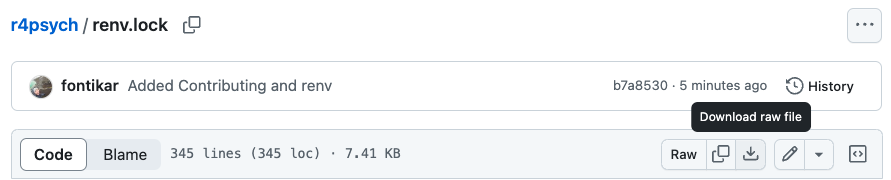
\includegraphics{images/renv.png}

Alternatively, you can
\href{https://happygitwithr.com/clone.html?q=clone\#clone}{clone} our
repository into your computer. Learn more about cloning repositorsies
and other GitHub workflows in \href{https://happygitwithr.com/}{Happy
Git} by Jenny Bryan.

Once you have this file downloaded, move it in a relevant
\href{}{project directory} and then we can let \texttt{\{renv\}} work
its magic.

\subsection{Install}\label{install}

First things first, lets install \texttt{renv} if we don't have it
already.

\begin{Shaded}
\begin{Highlighting}[]
\FunctionTok{install.packages}\NormalTok{(}\StringTok{"renv"}\NormalTok{)}

\FunctionTok{library}\NormalTok{(renv)}
\end{Highlighting}
\end{Shaded}

\subsection{Recreate virtual
enviroment}\label{recreate-virtual-enviroment}

Now let's tell \texttt{renv} where our downloaded \texttt{renv.lock}
file is. Specific the path to the file in the function
\texttt{restore()} and you are good to go!

\begin{Shaded}
\begin{Highlighting}[]
\FunctionTok{restore}\NormalTok{(}\AttributeTok{lockfile =} \StringTok{"path\_to\_renv.lock"}\NormalTok{)}
\end{Highlighting}
\end{Shaded}

\bookmarksetup{startatroot}

\chapter{Organise}\label{organise}

There are lots of reasons to use R and R Studio for your data analysis,
but reproducibility ranks high on the list. By writing code that reads,
wrangles, cleans, visualises, and analyses your data, you are
documenting the process that your data has been through from its raw
state through to its analysed state. Reproducibility is all about
someone else (or you in the future) being able to take your data and the
code you have written and use it to produce exactly the same analysis
values that you report in your paper or thesis.

With this goal in mind, there are a few best practices we recommend, to
ensure that your code is usable in the future, irrespective of what
machine it is being run on and by whom.

\section{R projects}\label{r-projects}

R really cares about where things live on your computer, even if you
don't. Humans have gotten out of the habit of thinking very hard about
where they put things on their machine; the search capabilities on the
modern computer are quite good and you can generally find files quite
easily by searching for them.

When you are coding in R, however, you need to explicitly tell R where
to find things. You can make this process much easier for yourself by
always working within an RStudio Project.

When you work within an RStudio project, you can reference everything in
relation to the top level of that project folder. It doesn't matter
where that project folder lives on your machine (i.e.~Desktop,
Documents, OneDrive, Dropbox) the code you write is always relative to
your project folder. This means that you can share that whole project
folder with someone else (your collaborators or supervisor), and your
code won't break.

\begin{quote}
When you start a new analysis project, create a New RStudio Project via
the File tab.
\end{quote}

\begin{figure}[H]

{\centering 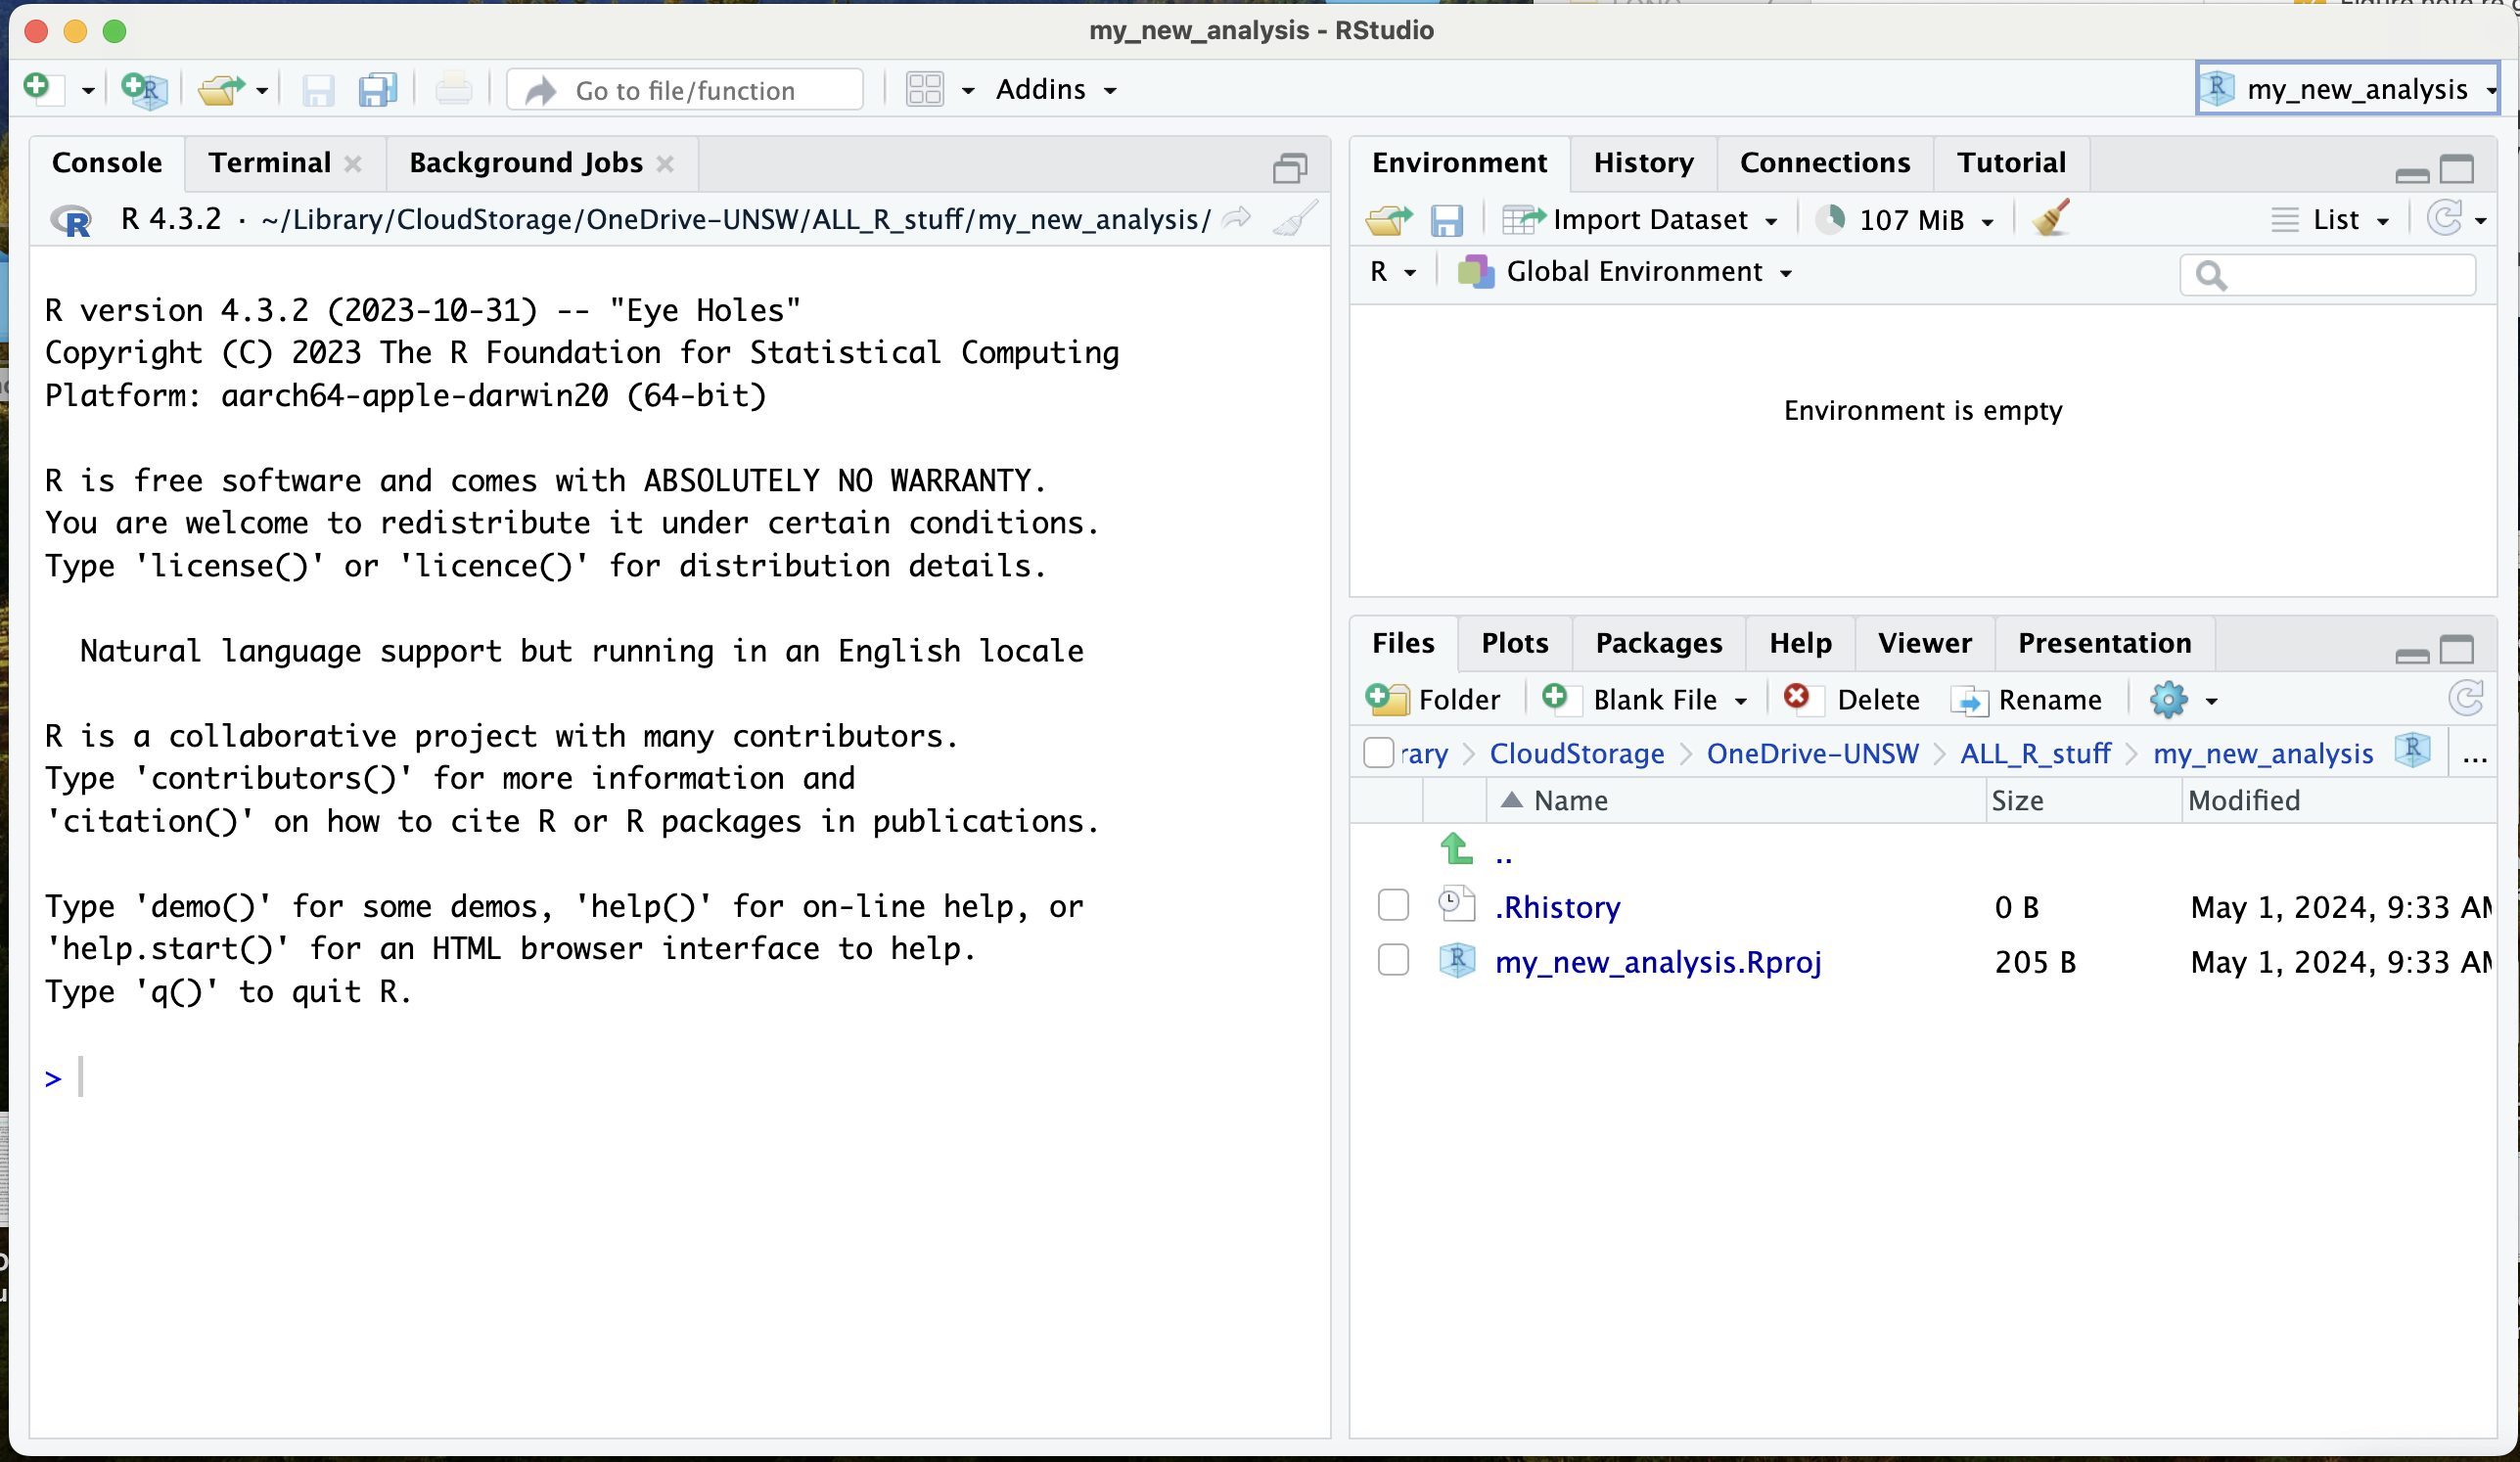
\includegraphics{images/project.png}

}

\caption{Working in an RStudio Project called my\_new\_analysis}

\end{figure}%

Always open RStudio by double clicking on the .RProj file in the folder
on your machine. There is an icon in the top right corner of RStudio
that shows you which project you are working in and makes it easy to
switch between projects.

\section{where is here?}\label{where-is-here}

Once you have set up a project to contain your analysis, you can avoid
further file path drama by using the \texttt{here()} package. This
package makes it super easy to refer to file paths and ensures that your
code will work, even if someone else is trying to run it on a different
computer.

Once you have installed the \texttt{here()} package, use it to tell R
where you find your data like this. This code chunk loads there
\texttt{here()} and \texttt{readr()} packages and then tells R to read
in a csv file, located in the ``data'' folder, and the file is called
file.csv

\begin{Shaded}
\begin{Highlighting}[]
\NormalTok{mydata }\OtherTok{\textless{}{-}} \FunctionTok{read\_csv}\NormalTok{(}\FunctionTok{here}\NormalTok{(}\StringTok{"data"}\NormalTok{, }\StringTok{"file.csv"}\NormalTok{))}
\end{Highlighting}
\end{Shaded}

By referring to the location of your data using the \texttt{here()}
package, here is no need worry about working directories, and you can be
sure that your code will work on any machine.

\begin{quote}
To read more about why projects and the \texttt{here()} package are
useful, check out
\href{https://www.tidyverse.org/blog/2017/12/workflow-vs-script/}{this
blog by Jenny Bryan}
\end{quote}

\section{folder structure}\label{folder-structure}

Once you have your project set up, you might like to think about
imposing some structure on it. It is mostly personal preference, but
many analysis projects include the following folders.

\begin{itemize}
\tightlist
\item
  data

  \begin{itemize}
  \tightlist
  \item
    raw-data
  \item
    clean-data
  \end{itemize}
\item
  output

  \begin{itemize}
  \tightlist
  \item
    figures
  \item
    tables
  \end{itemize}
\item
  manuscript
\end{itemize}

You always want to keep your raw data untouched and separate from any
data that you write back to your machine after your data cleaning
process, so a raw-data subfolder can be useful.

In addition, you might want to organise your figures and tables into an
output folder and put any writing that you are doing in the manuscripts
folder.

\begin{quote}
If you want to write a manuscript (or maybe your whole thesis!) using
RMarkdown, check out the \texttt{papaja} (Preparing APA Journal
Articles) package
\end{quote}

Usually the scripts (or R Markdown) documents that you write your code
in, live in the top level of your project file. In RStudio, your project
structure might look something like this.

\begin{figure}[H]

{\centering 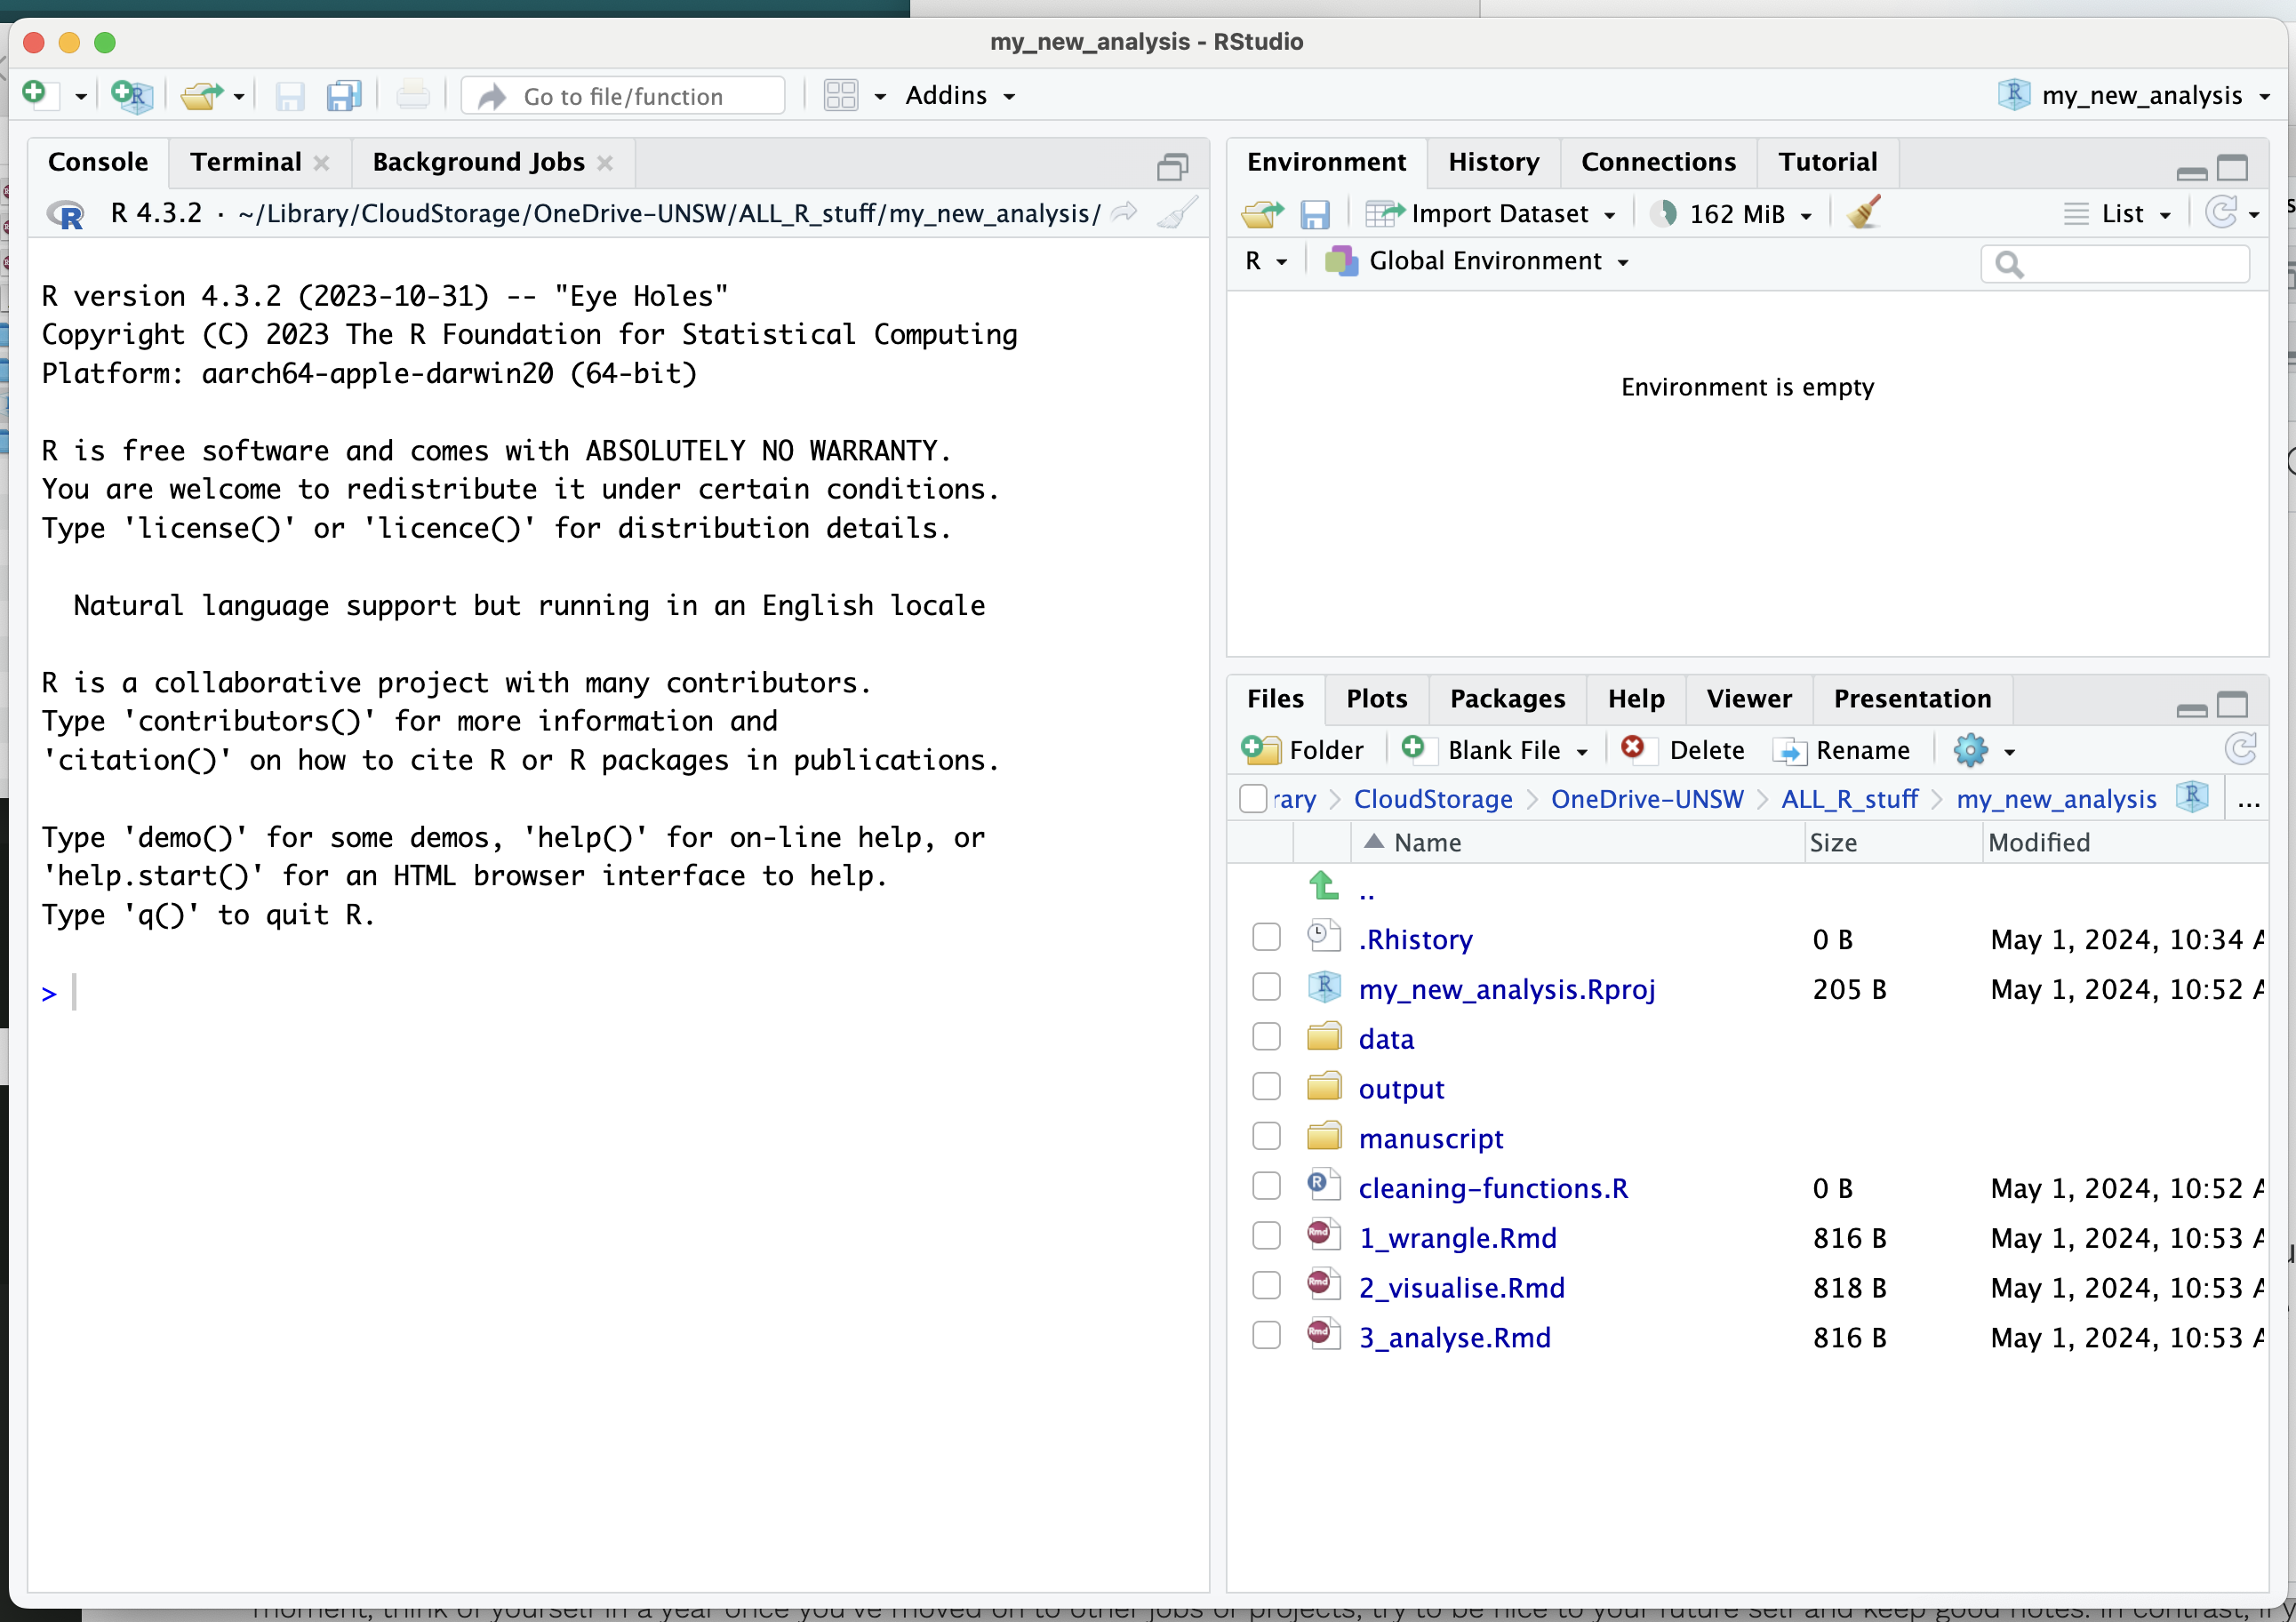
\includegraphics{images/structure.png}

}

\caption{A project structure template}

\end{figure}%

\section{naming things}\label{naming-things}

When naming things in your analysis folder, it is a good idea to think
about your future self. In all likelihood, when you come back to this
analysis in a few months time, you will have no recollection how it
actually worked, but you can leave yourself some breadcrumbs by being a
bit intentional about naming things.

Your file names should be meaningful and orderly. The name of each file
should tell the new user (or future you) what is in the file and where
it goes in the process.

\begin{itemize}
\tightlist
\item
  cleaning-functions.R
\item
  1\_wrangle.Rmd
\item
  2\_visualise.Rmd
\item
  3\_analyse.Rmd
\end{itemize}

In this project, I can tell by glancing at the file names that I have a
script (.R) that contains functions and three R Markdown files that
contain each stage of the analysis.

Sticking with lower case is a good idea; avoid special characters and
use - or \_ to fill any gaps.

Find more useful naming tips in the
\href{https://style.tidyverse.org/files.html}{Tidyverse Style guide}.

\section{documenting things}\label{documenting-things}

\subsection{README}\label{readme}

In addition to the breadcrumbs that our file names leave, it is also a
good idea to leave explicit notes to your future self (or someone else)
in a README.md file. This is a simple text file that contains
instructions for how the user should engage with your project.

Create a new Markdown file and save it as README.md

Use it to leave yourself instructions that look a bit like this.

\begin{figure}[H]

{\centering 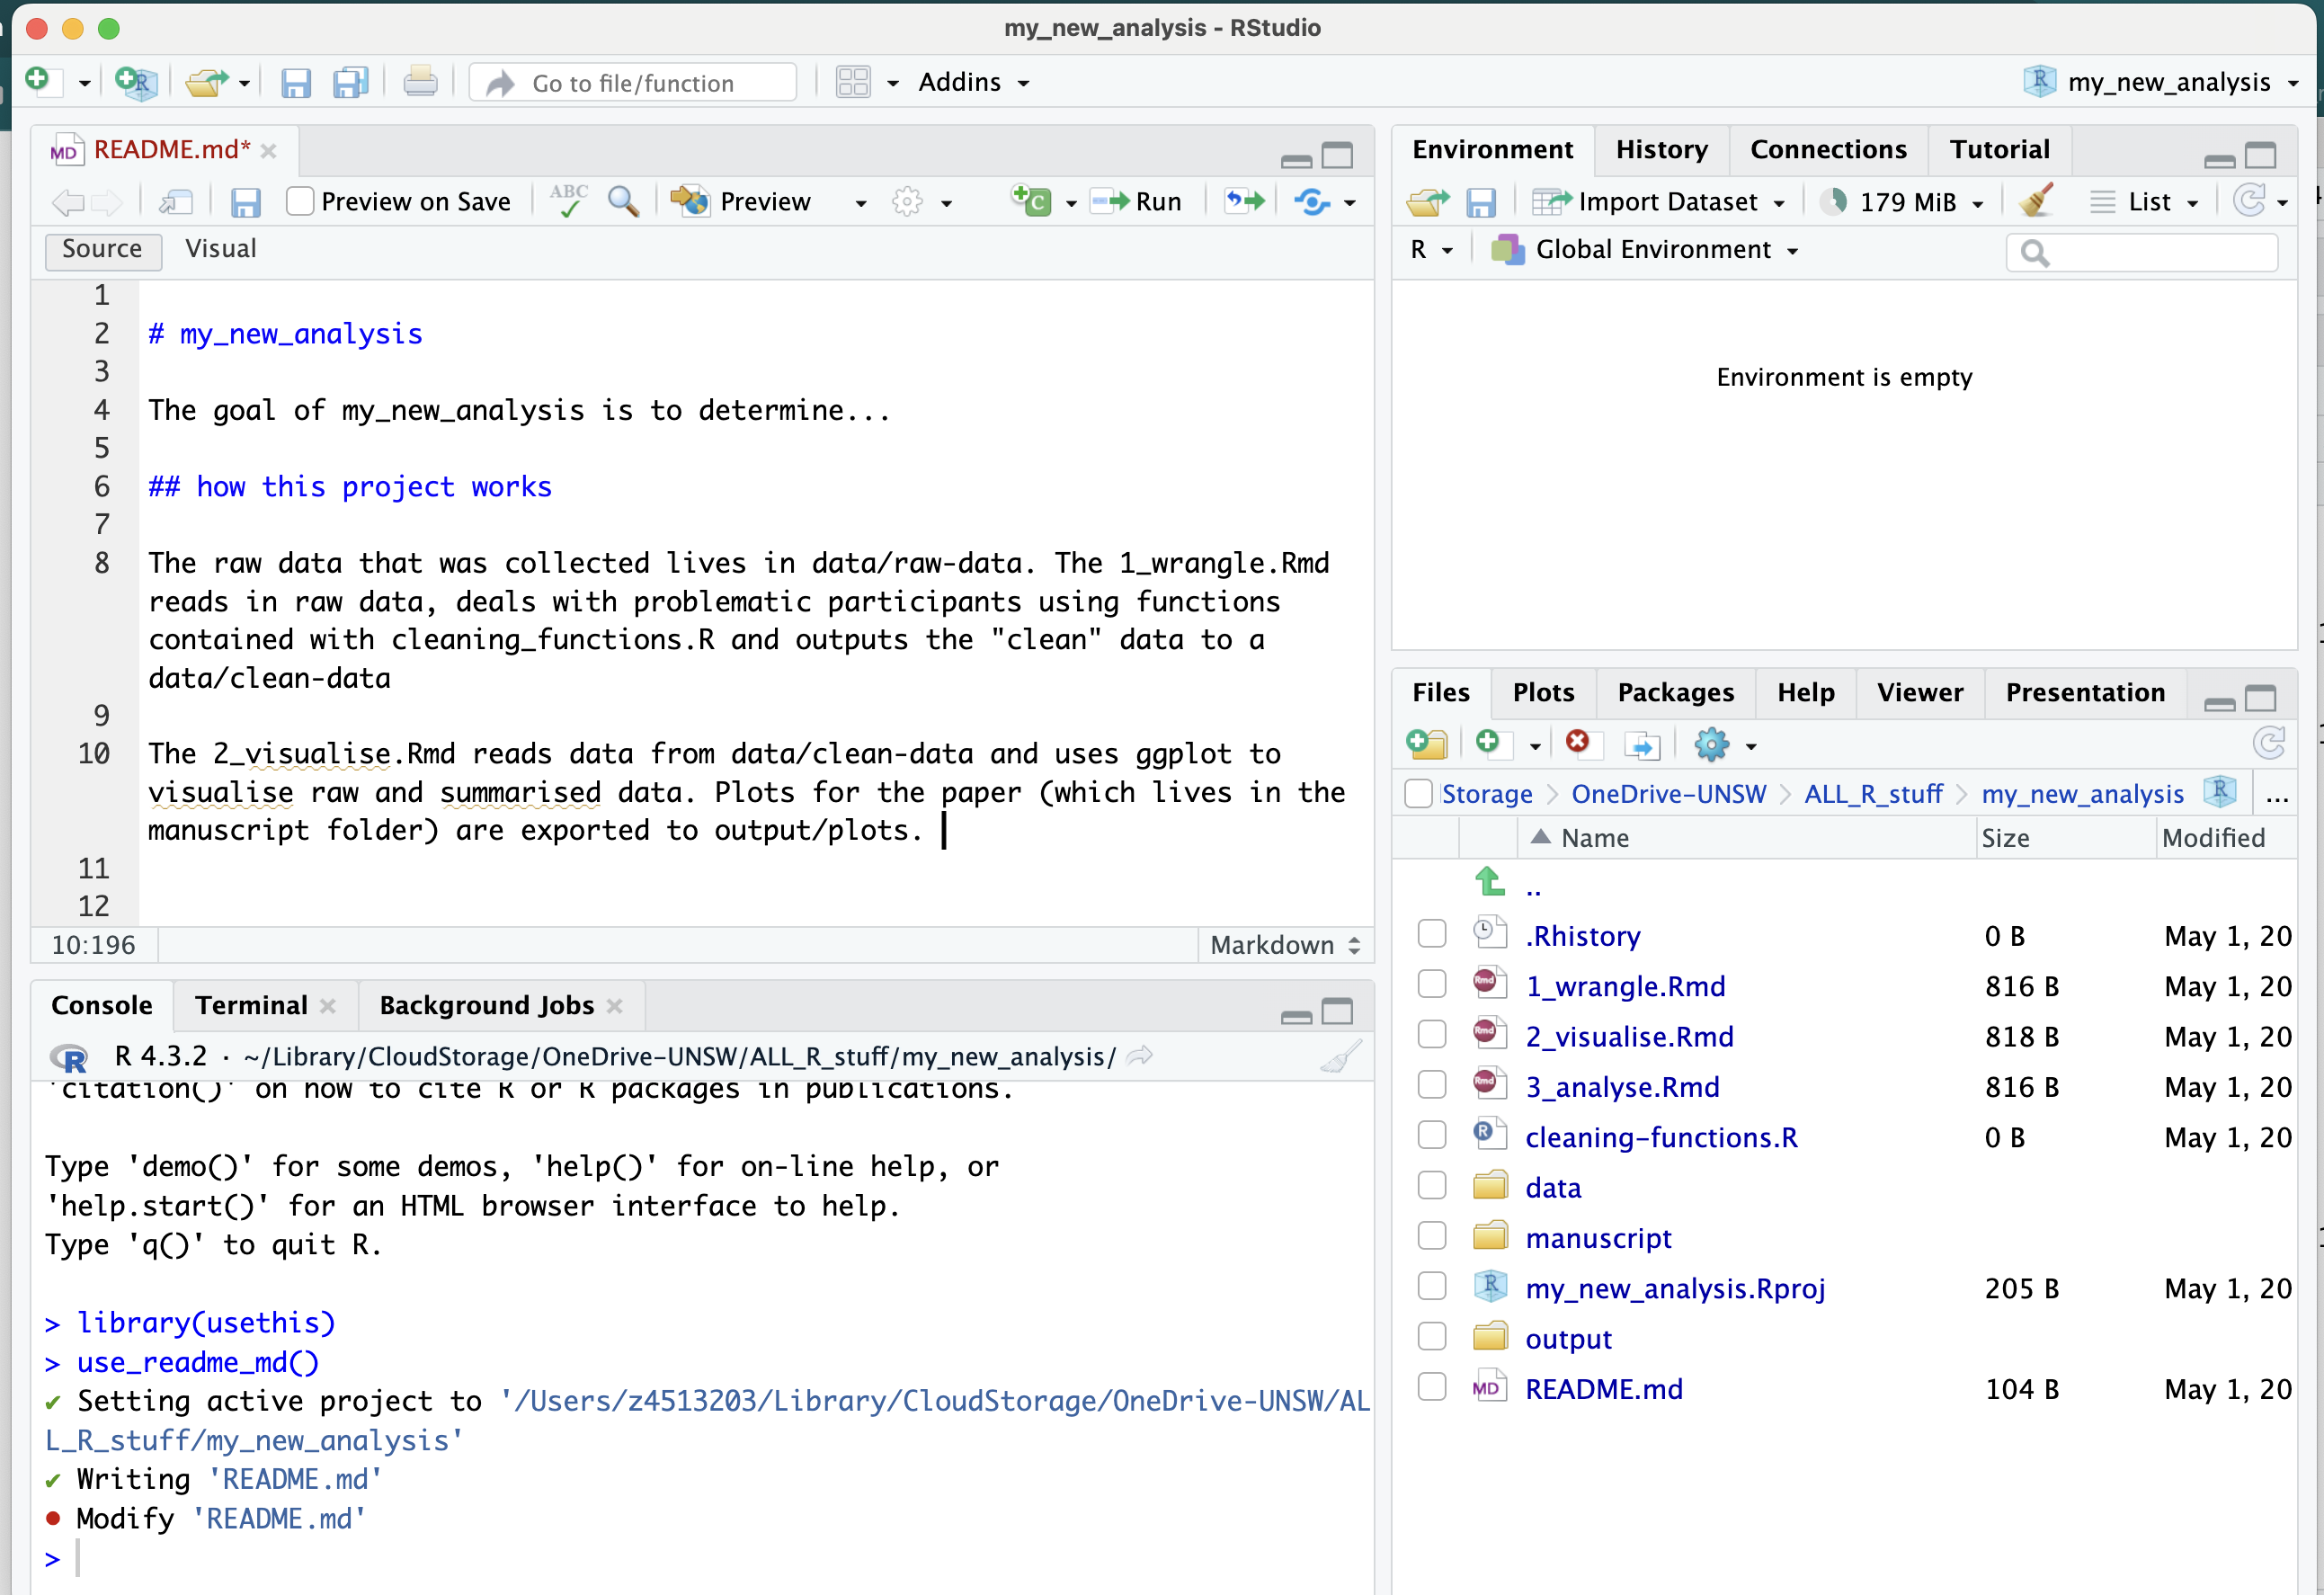
\includegraphics{images/readme.png}

}

\caption{An example README file}

\end{figure}%

\subsection{R Markdown}\label{r-markdown}

In addition to leaving your future self explicit notes about how to
engage with the project generally in a README document, it is also best
practice to document your code in a way that makes it really clear what
the code is doing and why. For this reason, we recommend using R
Markdown documents (rather than R scripts) for your analysis.

R Markdown is a handy file format that allows you to intersperse chunks
of code with notes. This kind of document makes it easy to write
explanations, interpretations, and thoughts for your future self as you
code. This kind of documentation makes it much more likely to be able to
make sense of what you have done and why, when you come back to your
analysis in a few months time.

R Markdown documents can also be ``knitted'' into html, pdf, or word
documents, allowing you to share your analysis (and associated thoughts)
with collaborators, even if they don't know R.

To get up to speed on R Markdown and how to use it, check out
RLadiesSydney
\href{https://rladiessydney.org/courses/ryouwithme/04-markymark-1/}{\#RYouWithMe
MarkyMark module}

\bookmarksetup{startatroot}

\chapter{Import}\label{import}

\section{Reading in Excel
spreadsheets}\label{reading-in-excel-spreadsheets}

This is

\subsection{Reading in .csv}\label{reading-in-.csv}

\section{Reading in SPSS}\label{reading-in-spss}

\section{Reading in Qualtrics data}\label{reading-in-qualtrics-data}

\subsection{Reading in .sav}\label{reading-in-.sav}

\bookmarksetup{startatroot}

\chapter{Read in the data}\label{read-in-the-data}

Remember the file setup described above? This is where that starts to be
important. Remember, our working directory (i.e., where R thinks
``here'' is) was set via the Rproj file -- so it is the ``Williams Lab
Core R'' folder. You can check this by typing \texttt{getwd()} or
\texttt{here()} in the console.

For most of this core script, we'll be using data from a file called
sampledata.sav, which should be in the data subfolder from the zipped
file. If not, sort that out now!

A .sav file is in SPSS format. When you export from Qualtrics into
.sav/SPSS format, it retains helpful information like question wording
and response labels. If you export straight to .csv, you lose that info
and will find yourself cross-checking back to Qualtrics. So, strong word
of advice to always export to .sav.

The code below uses the \texttt{here} command to direct R to the data
folder \emph{from the working directory}, and then the .sav file within
it.

The \texttt{glimpse} command gives a nice overview of the variables,
their type, and a preview of the data.

\begin{Shaded}
\begin{Highlighting}[]
\NormalTok{data }\OtherTok{\textless{}{-}} \FunctionTok{read\_sav}\NormalTok{(}\FunctionTok{here}\NormalTok{(}\StringTok{"data"}\NormalTok{, }\StringTok{"sampledata.sav"}\NormalTok{)) }

\FunctionTok{glimpse}\NormalTok{(data)}
\end{Highlighting}
\end{Shaded}

These variable names won't be very nice to work with with awkward and
inconsistent capitalisation. Actual Qualtrics exports are even messier!

The \texttt{clean\_names} function from \texttt{janitor} helps clean
them up!

\texttt{data\_cleanednames\ \textless{}-} at the start of the line saves
the change to a new dataframe. Alternately, you could write it back to
the same dataframe (e.g., \texttt{data\ \textless{}-} ), but this should
be done very intentionally as it makes it harder to backtrack to the
source of an error. The general rule is to create a new dataframe each
time you implement a big change on the data.

The \texttt{glimpse} command here shows you that you effectively cleaned
the variable names!

\begin{Shaded}
\begin{Highlighting}[]
\NormalTok{data\_cleanednames }\OtherTok{\textless{}{-}} \FunctionTok{clean\_names}\NormalTok{(data)}

\FunctionTok{glimpse}\NormalTok{(data\_cleanednames)}
\end{Highlighting}
\end{Shaded}

A few things about working with files in SPSS format (.sav) before we
continue. The reason why we bother with this is that the SPSS format
maximises the information in the file. Unlike exporting to .csv or
another spreadsheet format, .sav retains information about question
wording (saved as a variable label) and response labelling (saved as a
value label).

If you look at the variable types at the right of the \texttt{glimpse}
output, you'll see the some of the variables are dbl (numeric) while
some are dbl+lbl (numeric with labelled values). If you view the
\texttt{data} object (by clicking on it in the Environment or using
\texttt{view(data)}) you will see that some of the variables have the
question wording below the variable name.

Having this information on hand is really helpful when working with your
data!

The \texttt{view\_df} function from the \texttt{sjPlot} package creates
a really nicely formatted html file that includes variable names,
question wording, response options, and response labelling. This code
saves the html file to the \texttt{output\_files} folder using the
\texttt{here} package (which starts where your Rproj file is). This html
file is nice as a reference for your own use or to share with a
supervisor or collaborator!

\begin{Shaded}
\begin{Highlighting}[]
\FunctionTok{view\_df}\NormalTok{(data\_cleanednames)}

\FunctionTok{view\_df}\NormalTok{(data\_cleanednames, }\AttributeTok{file=}\FunctionTok{here}\NormalTok{(}\StringTok{"output\_files"}\NormalTok{,}\StringTok{"spsstest\_codebook.html"}\NormalTok{))}
\end{Highlighting}
\end{Shaded}

The \texttt{data\_dict} function from \texttt{surveytoolbox} makes a
dataframe with all the variable and response labels - similar to the
html created above, but this can be called upon later in R as it's now
part of the environment.

\begin{Shaded}
\begin{Highlighting}[]
\NormalTok{datadictionary }\OtherTok{\textless{}{-}}\NormalTok{ data\_cleanednames }\SpecialCharTok{\%\textgreater{}\%}
  \FunctionTok{data\_dict}\NormalTok{()}
\end{Highlighting}
\end{Shaded}

Let's say you just want to know the question wording or response labels
for a particular variable, you can do this via code rather than checking
the whole dataset. The \texttt{extract\_vallab} command from
\texttt{surveytoolbox} returns the value labels for a given variable.

\begin{Shaded}
\begin{Highlighting}[]
\NormalTok{data\_cleanednames }\SpecialCharTok{\%\textgreater{}\%}
  \FunctionTok{extract\_vallab}\NormalTok{(}\StringTok{"demographicscateg"}\NormalTok{)}
\end{Highlighting}
\end{Shaded}

There are (evidently) times when packages \emph{do not like} labelled
data. So, here are a few tools for removing labels from the
\texttt{haven} package. Keep these up your sleeve for problem solving
later! \texttt{zap\_labels} and \texttt{zap\_label} not surprisingly
removes the labels - the first removes the value labels and the second
removes the variable labels! The code below makes a new data dictionary
of the zapped dataframe and glimpses the new dataframe to confirm the
labels are gone.

\begin{Shaded}
\begin{Highlighting}[]
\NormalTok{data\_zapped }\OtherTok{\textless{}{-}}\NormalTok{ data\_cleanednames }\SpecialCharTok{\%\textgreater{}\%}
  \FunctionTok{zap\_labels}\NormalTok{() }\SpecialCharTok{\%\textgreater{}\%}
  \FunctionTok{zap\_label}\NormalTok{()}

\NormalTok{datadictionary\_zapped }\OtherTok{\textless{}{-}}\NormalTok{ data\_zapped }\SpecialCharTok{\%\textgreater{}\%}
  \FunctionTok{data\_dict}\NormalTok{()}

\FunctionTok{glimpse}\NormalTok{(data\_zapped)}
\end{Highlighting}
\end{Shaded}

For the rest of this script, we will work with the \emph{zapped}
dataframe. This is the recommended approach to save headaches with
errors down the line.

\bookmarksetup{startatroot}

\chapter{Wrangle}\label{wrangle}

\section{Clean names}\label{clean-names}

\section{Dealing with labels}\label{dealing-with-labels}

\section{Exclusions}\label{exclusions}

\texttt{mutate} \texttt{case\_when}

\texttt{filter}

\section{Creating scales and indexes}\label{creating-scales-and-indexes}

\texttt{group\_by} \texttt{summarise}

\texttt{row\_wise} \texttt{mutate}

\subsection{Checking reliabilty}\label{checking-reliabilty}

\bookmarksetup{startatroot}

\chapter{Describe}\label{describe}

\section{getting a feel for your
data}\label{getting-a-feel-for-your-data}

\texttt{str}

\texttt{glimpse}

\texttt{skimr}

\section{counting things}\label{counting-things}

\texttt{group\_by} + \texttt{summarise} + \texttt{count}

\texttt{n}

\texttt{tabyl}

\section{getting descriptives}\label{getting-descriptives}

\texttt{group\_by} + \texttt{summarise} + \texttt{mean} \& \texttt{sd}

\begin{Shaded}
\begin{Highlighting}[]
\NormalTok{scale1\_by\_condition12 }\OtherTok{\textless{}{-}}\NormalTok{ data\_scalescomputed }\SpecialCharTok{\%\textgreater{}\%}
  \FunctionTok{group\_by}\NormalTok{(condition12) }\SpecialCharTok{\%\textgreater{}\%}
  \FunctionTok{summarise}\NormalTok{(}\AttributeTok{mean\_scale1 =} \FunctionTok{mean}\NormalTok{(scale1\_index, }\AttributeTok{na.rm =} \ConstantTok{TRUE}\NormalTok{),}
            \AttributeTok{sd\_scale1 =} \FunctionTok{sd}\NormalTok{(scale1\_index, }\AttributeTok{na.rm =} \ConstantTok{TRUE}\NormalTok{))}
\end{Highlighting}
\end{Shaded}

\subsection{Three things to remember}\label{three-things-to-remember}

\begin{enumerate}
\def\labelenumi{\arabic{enumi}.}
\tightlist
\item
  When we compute means, we need to set the decimals via
  \texttt{round()}.
\item
  We also need to tell R to calculate the mean, even if some of the
  contributing data points are missing. This is what
  \texttt{na.rm\ =\ TRUE} does.
\item
  As noted above, \texttt{rowwise} asks R to do something for each row
  (which is what we want here -- to compute the mean of the contributing
  items for each participant). Whenever we use \texttt{rowwise} (or
  \texttt{group\_by}), we need to \texttt{ungroup()} at the end to avoid
  issues down the line.
\end{enumerate}

\section{tables??}\label{tables}

\texttt{gt}

\begin{Shaded}
\begin{Highlighting}[]
\FunctionTok{gt}\NormalTok{(scale1\_by\_condition12)}
\end{Highlighting}
\end{Shaded}

\texttt{apaTable}

\bookmarksetup{startatroot}

\chapter{Plot}\label{plot}

\section{Plotting raw data}\label{plotting-raw-data}

\texttt{geom\_point}

\texttt{geom\_histogram}

\texttt{geom\_boxplot}

\texttt{geom\_violin}

\section{Plotting data summaries}\label{plotting-data-summaries}

\texttt{geom\_col}

\bookmarksetup{startatroot}

\chapter{Infer}\label{infer}

\bookmarksetup{startatroot}

\chapter{Moving into analyses}\label{moving-into-analyses}

\begin{quote}
thoughts from Jenny : I wonder whether it would be useful to structure
this in terms of lets combine skills from previous chapters to..
\end{quote}

\begin{enumerate}
\def\labelenumi{\arabic{enumi}.}
\tightlist
\item
  ask a question,
\item
  get plots/descriptives
\item
  then answer it with inferentials?
\item
  And repeat that process for t-test, linear regression and anova?
\end{enumerate}

\section{Plots and descriptives}\label{plots-and-descriptives}

Now, let's test whether this scale varies by condition (condition 1
vs.~condition 2 in condition12).

Before jumping into t-tests, let's first visualise the data
(scale1\_index) to get a sense of what it looks like.

The first command here tells R to treat condition12 as a categorical
variable that groups the data (technically, a factor). This is helpful
for plotting. The code uses the \texttt{dataframe\$variablename}
structure to do a command on just one variable.

The second command pipes the data into a command to create a boxplot
(\texttt{geom\_boxplot}) with the datapoints plotted as well
(\texttt{geom\_jitter}).The \texttt{width} command makes the plotting of
the dots a bit narrower to help with interpretation.

\begin{Shaded}
\begin{Highlighting}[]
\NormalTok{data\_scalescomputed}\SpecialCharTok{$}\NormalTok{condition12 }\OtherTok{\textless{}{-}} \FunctionTok{as.factor}\NormalTok{(data\_scalescomputed}\SpecialCharTok{$}\NormalTok{condition12)}

\NormalTok{data\_scalescomputed }\SpecialCharTok{\%\textgreater{}\%}
  \FunctionTok{ggplot}\NormalTok{(}\FunctionTok{aes}\NormalTok{(}\AttributeTok{x =}\NormalTok{ condition12, }\AttributeTok{y =}\NormalTok{ scale1\_index, }\AttributeTok{fill =}\NormalTok{ condition12)) }\SpecialCharTok{+}
  \FunctionTok{geom\_boxplot}\NormalTok{(}\AttributeTok{alpha =}\NormalTok{ .}\DecValTok{5}\NormalTok{) }\SpecialCharTok{+}
  \FunctionTok{geom\_jitter}\NormalTok{(}\AttributeTok{alpha =}\NormalTok{ .}\DecValTok{5}\NormalTok{, }\AttributeTok{width =} \FloatTok{0.2}\NormalTok{)}
\end{Highlighting}
\end{Shaded}

Based on the boxplot, we'd expect a t-test to be nonsignificant - the
wide boxes of the plots for each condition overlap, even though the mean
of condition 2 is slightly higher than condition 1 (the horizontal line
through the box).

\section{t-test}\label{t-test}

The first line of code uses the base R command to run a t-test. It tells
R to do the test on the \texttt{data\_scalescomputed} data frame, asking
whether \texttt{scale1\_index} varies by (\textasciitilde) condition.
\texttt{var.} sets the assumption of variance and \texttt{conf.level}
sets the desired alpha of the test. That command is wrapped in the handy
\texttt{t\_apa} function, which makes the output much easier to read
(and pull directly into a write-up!), and also allows us to get a
confidence interval on the effect size (\texttt{es\_ci}).

For reporting, you'd probably also want to know the means and standard
deviations by condition. The next bit of code asks R to do this, using
the \texttt{summarise} function, separately for each condition. Reminder
to use \texttt{na.rm} here to account for any missing values.

The \texttt{gt()} command shows the requested dataframe in a nice
formatting.

\begin{Shaded}
\begin{Highlighting}[]
\FunctionTok{t\_apa}\NormalTok{(}\FunctionTok{t.test}\NormalTok{(}\AttributeTok{data =}\NormalTok{ data\_scalescomputed, scale1\_index }\SpecialCharTok{\textasciitilde{}}\NormalTok{ condition12, }\AttributeTok{var. =} \ConstantTok{TRUE}\NormalTok{, }\AttributeTok{conf.level =}\NormalTok{ .}\DecValTok{95}\NormalTok{), }\AttributeTok{es\_ci =} \ConstantTok{TRUE}\NormalTok{)}


\NormalTok{scale1\_by\_condition12 }\OtherTok{\textless{}{-}}\NormalTok{ data\_scalescomputed }\SpecialCharTok{\%\textgreater{}\%}
  \FunctionTok{group\_by}\NormalTok{(condition12) }\SpecialCharTok{\%\textgreater{}\%}
  \FunctionTok{summarise}\NormalTok{(}\AttributeTok{mean\_scale1 =} \FunctionTok{mean}\NormalTok{(scale1\_index, }\AttributeTok{na.rm =} \ConstantTok{TRUE}\NormalTok{),}
            \AttributeTok{sd\_scale1 =} \FunctionTok{sd}\NormalTok{(scale1\_index, }\AttributeTok{na.rm =} \ConstantTok{TRUE}\NormalTok{))}


\FunctionTok{gt}\NormalTok{(scale1\_by\_condition12)}
\end{Highlighting}
\end{Shaded}

\bookmarksetup{startatroot}

\chapter{Linear regression}\label{linear-regression}

\emph{lw\_addnarrativehere}

\begin{itemize}
\tightlist
\item
  outcome: variable\_6
\item
  step 1: demographics\_categ
\item
  step 2: variable\_4
\item
  step 3: scale1\_index
\end{itemize}

this asks the lm package to use predictor to predict outcome

lm(outcome \textasciitilde{} predictor )

\begin{Shaded}
\begin{Highlighting}[]
\NormalTok{regression1 }\OtherTok{\textless{}{-}} \FunctionTok{lm}\NormalTok{(}\AttributeTok{data =}\NormalTok{ data\_scalescomputed, variable6 }\SpecialCharTok{\textasciitilde{}}\NormalTok{ demographicscateg }\SpecialCharTok{+}\NormalTok{ variable4 }\SpecialCharTok{+}\NormalTok{ scale1\_index)}

\FunctionTok{summary}\NormalTok{(regression1)}
\end{Highlighting}
\end{Shaded}

\emph{lw\_addnarrativehere} simulates hierarchical stepwise regression?

\begin{Shaded}
\begin{Highlighting}[]
\NormalTok{regressionlm1 }\OtherTok{\textless{}{-}} \FunctionTok{lm}\NormalTok{(}\AttributeTok{data =}\NormalTok{ data\_scalescomputed, variable6 }\SpecialCharTok{\textasciitilde{}}\NormalTok{ demographicscateg)}
\NormalTok{regressionlm2 }\OtherTok{\textless{}{-}} \FunctionTok{lm}\NormalTok{(}\AttributeTok{data =}\NormalTok{ data\_scalescomputed, variable6 }\SpecialCharTok{\textasciitilde{}}\NormalTok{ demographicscateg }\SpecialCharTok{+}\NormalTok{ variable4)}
\NormalTok{regressionlm3 }\OtherTok{\textless{}{-}} \FunctionTok{lm}\NormalTok{(}\AttributeTok{data =}\NormalTok{ data\_scalescomputed, variable6 }\SpecialCharTok{\textasciitilde{}}\NormalTok{ demographicscateg }\SpecialCharTok{+}\NormalTok{ variable4 }\SpecialCharTok{+}\NormalTok{ scale1\_index)}

\FunctionTok{summary}\NormalTok{(regressionlm1)}
\FunctionTok{summary}\NormalTok{(regressionlm2)}
\FunctionTok{summary}\NormalTok{(regressionlm3)}


\FunctionTok{apa.reg.table}\NormalTok{(regressionlm1, regressionlm2, regressionlm3, }\AttributeTok{filename =} \FunctionTok{here}\NormalTok{(}\StringTok{"output\_files"}\NormalTok{,}\StringTok{"RegressionTable3\_APA.doc"}\NormalTok{), }\AttributeTok{table.number =} \DecValTok{3}\NormalTok{)}

\FunctionTok{report}\NormalTok{(regressionlm3)}
\end{Highlighting}
\end{Shaded}

\bookmarksetup{startatroot}

\chapter{Analysis of Variance (ANOVA)}\label{analysis-of-variance-anova}

\emph{lw add narrative}

4 (between participants - condition1234) x2 (between participants -
individual difference categorical variable - demographicscateg) design

outcome: scale1\_index

\begin{Shaded}
\begin{Highlighting}[]
\DocumentationTok{\#\# first tell R that condition and demographicscateg are categorical (factors)}

\NormalTok{data\_scalescomputed}\SpecialCharTok{$}\NormalTok{condition1234 }\OtherTok{\textless{}{-}} \FunctionTok{as.factor}\NormalTok{(data\_scalescomputed}\SpecialCharTok{$}\NormalTok{condition1234)}
\NormalTok{data\_scalescomputed}\SpecialCharTok{$}\NormalTok{demographicscateg }\OtherTok{\textless{}{-}} \FunctionTok{as.factor}\NormalTok{(data\_scalescomputed}\SpecialCharTok{$}\NormalTok{demographicscateg)}

\DocumentationTok{\#\# this creates a dataframe that contains the summary statistics (means, standard deviations, etc.)}

\NormalTok{scale1\_stats }\OtherTok{\textless{}{-}} \FunctionTok{ezStats}\NormalTok{(}\AttributeTok{data =}\NormalTok{ data\_scalescomputed, }
                            \AttributeTok{dv =}\NormalTok{ scale1\_index,}
                            \AttributeTok{wid =}\NormalTok{ participantid,}
                            \AttributeTok{between =} \FunctionTok{c}\NormalTok{(}\StringTok{"condition1234"}\NormalTok{,}\StringTok{"demographicscateg"}\NormalTok{))}
                            
\FunctionTok{print}\NormalTok{(scale1\_stats)}

\DocumentationTok{\#\# this carries out an anova with condition1234 and demographicscateg as between{-}participants factors}
\DocumentationTok{\#\# the output includes statistical tests of the main effect of condition1234, the main effect of demographicscateg, and the interaction between the two}

\NormalTok{scale1\_anova }\OtherTok{\textless{}{-}} \FunctionTok{ezANOVA}\NormalTok{(}\AttributeTok{data =}\NormalTok{ data\_scalescomputed, }
                            \AttributeTok{dv =}\NormalTok{ scale1\_index,}
                            \AttributeTok{wid =}\NormalTok{ participantid,}
                            \AttributeTok{between =} \FunctionTok{c}\NormalTok{(}\StringTok{"condition1234"}\NormalTok{,}\StringTok{"demographicscateg"}\NormalTok{),}
                            \AttributeTok{return\_aov =} \ConstantTok{TRUE}\NormalTok{)}

\FunctionTok{print}\NormalTok{(scale1\_anova)}

\DocumentationTok{\#\# }\AlertTok{NOTE}\DocumentationTok{ THAT THE FOLLOWING WOULD BE DONE TO FURTHER INVESTIGATE AN INTERACTION OR A DIFFERENCE IN A MULTI{-}CATEGORICAL VARIABLE. }
\DocumentationTok{\#\# to build the contrasts we want to do (e.g., baseline vs. midpoint for PhD), we need to ask emmeans to create output to see what the rows represent.}

\NormalTok{scale1\_emm }\OtherTok{\textless{}{-}} \FunctionTok{emmeans}\NormalTok{(scale1\_anova}\SpecialCharTok{$}\NormalTok{aov, }\SpecialCharTok{\textasciitilde{}}\NormalTok{ condition1234 }\SpecialCharTok{*}\NormalTok{ demographicscateg)}

\NormalTok{scale1\_emm}

\DocumentationTok{\#\# now we can create a set of named vectors that represent each of the 8 means, based on the position in the 8{-}item list from emmeans.}

\NormalTok{cond1categ1 }\OtherTok{=} \FunctionTok{c}\NormalTok{(}\DecValTok{1}\NormalTok{,}\DecValTok{0}\NormalTok{,}\DecValTok{0}\NormalTok{,}\DecValTok{0}\NormalTok{,}\DecValTok{0}\NormalTok{,}\DecValTok{0}\NormalTok{,}\DecValTok{0}\NormalTok{,}\DecValTok{0}\NormalTok{)}
\NormalTok{cond2categ1 }\OtherTok{=} \FunctionTok{c}\NormalTok{(}\DecValTok{0}\NormalTok{,}\DecValTok{1}\NormalTok{,}\DecValTok{0}\NormalTok{,}\DecValTok{0}\NormalTok{,}\DecValTok{0}\NormalTok{,}\DecValTok{0}\NormalTok{,}\DecValTok{0}\NormalTok{,}\DecValTok{0}\NormalTok{)}
\NormalTok{cond3categ1 }\OtherTok{=} \FunctionTok{c}\NormalTok{(}\DecValTok{0}\NormalTok{,}\DecValTok{0}\NormalTok{,}\DecValTok{1}\NormalTok{,}\DecValTok{0}\NormalTok{,}\DecValTok{0}\NormalTok{,}\DecValTok{0}\NormalTok{,}\DecValTok{0}\NormalTok{,}\DecValTok{0}\NormalTok{)}
\NormalTok{cond4categ1 }\OtherTok{=} \FunctionTok{c}\NormalTok{(}\DecValTok{0}\NormalTok{,}\DecValTok{0}\NormalTok{,}\DecValTok{0}\NormalTok{,}\DecValTok{1}\NormalTok{,}\DecValTok{0}\NormalTok{,}\DecValTok{0}\NormalTok{,}\DecValTok{0}\NormalTok{,}\DecValTok{0}\NormalTok{)}
\NormalTok{cond1categ2 }\OtherTok{=} \FunctionTok{c}\NormalTok{(}\DecValTok{0}\NormalTok{,}\DecValTok{0}\NormalTok{,}\DecValTok{0}\NormalTok{,}\DecValTok{0}\NormalTok{,}\DecValTok{1}\NormalTok{,}\DecValTok{0}\NormalTok{,}\DecValTok{0}\NormalTok{,}\DecValTok{0}\NormalTok{)}
\NormalTok{cond2categ2 }\OtherTok{=} \FunctionTok{c}\NormalTok{(}\DecValTok{0}\NormalTok{,}\DecValTok{0}\NormalTok{,}\DecValTok{0}\NormalTok{,}\DecValTok{0}\NormalTok{,}\DecValTok{0}\NormalTok{,}\DecValTok{1}\NormalTok{,}\DecValTok{0}\NormalTok{,}\DecValTok{0}\NormalTok{)}
\NormalTok{cond3categ2 }\OtherTok{=} \FunctionTok{c}\NormalTok{(}\DecValTok{0}\NormalTok{,}\DecValTok{0}\NormalTok{,}\DecValTok{0}\NormalTok{,}\DecValTok{0}\NormalTok{,}\DecValTok{0}\NormalTok{,}\DecValTok{0}\NormalTok{,}\DecValTok{1}\NormalTok{,}\DecValTok{0}\NormalTok{)}
\NormalTok{cond4categ2 }\OtherTok{=} \FunctionTok{c}\NormalTok{(}\DecValTok{0}\NormalTok{,}\DecValTok{0}\NormalTok{,}\DecValTok{0}\NormalTok{,}\DecValTok{0}\NormalTok{,}\DecValTok{0}\NormalTok{,}\DecValTok{0}\NormalTok{,}\DecValTok{0}\NormalTok{,}\DecValTok{1}\NormalTok{)}

\NormalTok{cond1 }\OtherTok{=} \FunctionTok{c}\NormalTok{(}\DecValTok{1}\NormalTok{,}\DecValTok{0}\NormalTok{,}\DecValTok{0}\NormalTok{,}\DecValTok{0}\NormalTok{,}\DecValTok{1}\NormalTok{,}\DecValTok{0}\NormalTok{,}\DecValTok{0}\NormalTok{,}\DecValTok{0}\NormalTok{)}
\NormalTok{cond2 }\OtherTok{=} \FunctionTok{c}\NormalTok{(}\DecValTok{0}\NormalTok{,}\DecValTok{1}\NormalTok{,}\DecValTok{0}\NormalTok{,}\DecValTok{0}\NormalTok{,}\DecValTok{0}\NormalTok{,}\DecValTok{1}\NormalTok{,}\DecValTok{0}\NormalTok{,}\DecValTok{0}\NormalTok{)}
\NormalTok{cond3 }\OtherTok{=} \FunctionTok{c}\NormalTok{(}\DecValTok{0}\NormalTok{,}\DecValTok{0}\NormalTok{,}\DecValTok{1}\NormalTok{,}\DecValTok{0}\NormalTok{,}\DecValTok{0}\NormalTok{,}\DecValTok{0}\NormalTok{,}\DecValTok{1}\NormalTok{,}\DecValTok{0}\NormalTok{)}
\NormalTok{cond4 }\OtherTok{=} \FunctionTok{c}\NormalTok{(}\DecValTok{0}\NormalTok{,}\DecValTok{0}\NormalTok{,}\DecValTok{0}\NormalTok{,}\DecValTok{1}\NormalTok{,}\DecValTok{0}\NormalTok{,}\DecValTok{0}\NormalTok{,}\DecValTok{0}\NormalTok{,}\DecValTok{1}\NormalTok{)}


\DocumentationTok{\#\# now we can ask for contrasts based on these vectors; we will explore the main effect of condition1234 by comparing each of the conditions to one another}

\NormalTok{scale1\_contrasts }\OtherTok{\textless{}{-}} \FunctionTok{contrast}\NormalTok{(scale1\_emm, }\AttributeTok{method =} \FunctionTok{list}\NormalTok{(}\StringTok{"cond1 {-} cond2"} \OtherTok{=}\NormalTok{ cond1 }\SpecialCharTok{{-}}\NormalTok{ cond2,}
                                       \StringTok{"cond1 {-} cond3"} \OtherTok{=}\NormalTok{ cond1 }\SpecialCharTok{{-}}\NormalTok{ cond3,}
                                       \StringTok{"cond1 {-} cond4"} \OtherTok{=}\NormalTok{ cond1 }\SpecialCharTok{{-}}\NormalTok{ cond4,}
                                       \StringTok{"cond2 {-} cond3"} \OtherTok{=}\NormalTok{ cond2 }\SpecialCharTok{{-}}\NormalTok{ cond3,}
                                       \StringTok{"cond2 {-} cond4"} \OtherTok{=}\NormalTok{ cond2 }\SpecialCharTok{{-}}\NormalTok{ cond4,}
                                       \StringTok{"cond3 {-} cond4"} \OtherTok{=}\NormalTok{ cond3 }\SpecialCharTok{{-}}\NormalTok{ cond4)) }
  

\NormalTok{scale1\_contrasts}

\DocumentationTok{\#\# here\textquotesingle{}s a version with confidence intervals instead of t and p values}

\NormalTok{scale1\_contrastsCI }\OtherTok{\textless{}{-}}\NormalTok{ scale1\_contrasts }\SpecialCharTok{\%\textgreater{}\%}
                          \FunctionTok{confint}\NormalTok{()}

\NormalTok{scale1\_contrastsCI}

\CommentTok{\#you may have a specific planned contrast to run. Here let\textquotesingle{}s imagine you want to compare condition 2 to all of the other 3 conditions in one comparison.}

\NormalTok{scale1\_plannedcontraststats }\OtherTok{\textless{}{-}} \FunctionTok{ezStats}\NormalTok{(}\AttributeTok{data =}\NormalTok{ data\_scalescomputed, }
                            \AttributeTok{dv =}\NormalTok{ scale1\_index,}
                            \AttributeTok{wid =}\NormalTok{ participantid,}
                            \AttributeTok{between =} \FunctionTok{c}\NormalTok{(}\StringTok{"condition1234"}\NormalTok{))}

\NormalTok{scale1\_plannedcontraststats}

\NormalTok{cond2v134 }\OtherTok{=} \FunctionTok{c}\NormalTok{(}\DecValTok{0}\NormalTok{,}\DecValTok{1}\NormalTok{,}\DecValTok{0}\NormalTok{,}\DecValTok{0}\NormalTok{,}\DecValTok{0}\NormalTok{,}\DecValTok{1}\NormalTok{,}\DecValTok{0}\NormalTok{,}\DecValTok{0}\NormalTok{)}
\NormalTok{cond134v2 }\OtherTok{=} \FunctionTok{c}\NormalTok{(}\DecValTok{1}\NormalTok{,}\DecValTok{0}\NormalTok{,}\DecValTok{1}\NormalTok{,}\DecValTok{1}\NormalTok{,}\DecValTok{1}\NormalTok{,}\DecValTok{0}\NormalTok{,}\DecValTok{1}\NormalTok{,}\DecValTok{1}\NormalTok{)}

\NormalTok{scale1\_plannedcontrasts }\OtherTok{\textless{}{-}} \FunctionTok{contrast}\NormalTok{(scale1\_emm, }\AttributeTok{method =} \FunctionTok{list}\NormalTok{(}\StringTok{"condition 1 vs all the rest"} \OtherTok{=}\NormalTok{ cond2v134 }\SpecialCharTok{{-}}\NormalTok{ cond134v2))}
  
\NormalTok{scale1\_plannedcontrasts}
\end{Highlighting}
\end{Shaded}

Let's make a figure!

\begin{Shaded}
\begin{Highlighting}[]
\NormalTok{data\_scalescomputed }\SpecialCharTok{\%\textgreater{}\%}
  \FunctionTok{ggplot}\NormalTok{(}\FunctionTok{aes}\NormalTok{(}\AttributeTok{x =}\NormalTok{ condition1234, }\AttributeTok{y =}\NormalTok{ scale1\_index, }\AttributeTok{fill =}\NormalTok{ demographicscateg)) }\SpecialCharTok{+}
  \FunctionTok{geom\_boxplot}\NormalTok{() }\SpecialCharTok{+}
  \FunctionTok{theme\_light}\NormalTok{()}


\NormalTok{data\_scalescomputed }\SpecialCharTok{\%\textgreater{}\%}
  \FunctionTok{ggplot}\NormalTok{(}\FunctionTok{aes}\NormalTok{(}\AttributeTok{x =}\NormalTok{ condition1234, }\AttributeTok{y =}\NormalTok{ scale1\_index)) }\SpecialCharTok{+}
  \FunctionTok{geom\_boxplot}\NormalTok{() }\SpecialCharTok{+}
  \FunctionTok{theme\_light}\NormalTok{()}
\end{Highlighting}
\end{Shaded}

\bookmarksetup{startatroot}

\chapter{Contributing}\label{contributing}

This resource is created in mind so that the community that uses it, can
also contribute to it. We hope this mindset will encourage the resource
to grow and stay up-to-date for R learners.

Importantly, \textbf{all skill levels} are welcome to contribute, even
if you think your skills are not up to scratch - this is what this guide
is for!

\subsection{GitHub Workflow}\label{github-workflow}

\subsection{Hello Quarto!}\label{hello-quarto}

This book is built by \href{https://quarto.org/}{Quarto} which is an
open source, cross-language publishing system that allows users to build
beautiful things from blogs, to websites and books!

You can learn more about the capabilities of Quarto in
\href{https://www.youtube.com/watch?v=p7Hxu4coDl8}{this talk} by Mine
Çetinkaya-Rundel \& Julia Stewart Lowndes at posit::conf(2023)

\subsubsection{Install Quarto}\label{install-quarto}

Let's first make sure we the latest version of
\href{https://quarto.org/docs/get-started/}{Quarto} installed.

\subsection{Quarto Workflow}\label{quarto-workflow}

\section{Book Structure}\label{book-structure}

\section{Book Practices and
Conventions}\label{book-practices-and-conventions}

\section{Book Contributions}\label{book-contributions}

\subsection{Edits}\label{edits}

\subsection{Additions}\label{additions}

\section{Contribution Review}\label{contribution-review}

\bookmarksetup{startatroot}

\chapter{Data}\label{data}

\bookmarksetup{startatroot}

\chapter{Appendix}\label{appendix}

\bookmarksetup{startatroot}

\chapter{how to install R and RStudio on your
machine}\label{how-to-install-r-and-rstudio-on-your-machine}

The marvellous Danielle Navarro has LOTS of useful R learning resources
on her YouTube channel.
\href{https://www.youtube.com/playlist?list=PLRPB0ZzEYegOZivdelOuEn-R-XUN-DOjd}{This
playlist} about how to install R and RStudio is particularly useful; no
matter which operating system you are dealing with\ldots{} Dani has you
covered.

\bookmarksetup{startatroot}

\chapter{how to install packages}\label{how-to-install-packages}

You only need to install a package once on your machine. Once the
package is installed, you will need to use \texttt{library()} to load
the functions in it every time you want to use it, but the installation
is a one time job. So you can either do it in the console, or using the
packages tab.

\section{option 1}\label{option-1}

Install a package by typing the following command with the name of the
package you would like to install in the console.

\begin{verbatim}
install.packages("packagename")
\end{verbatim}

\section{option 2}\label{option-2}

Alternatively, search for the package you would like to install in the
packages tab.

\begin{figure}[H]

{\centering 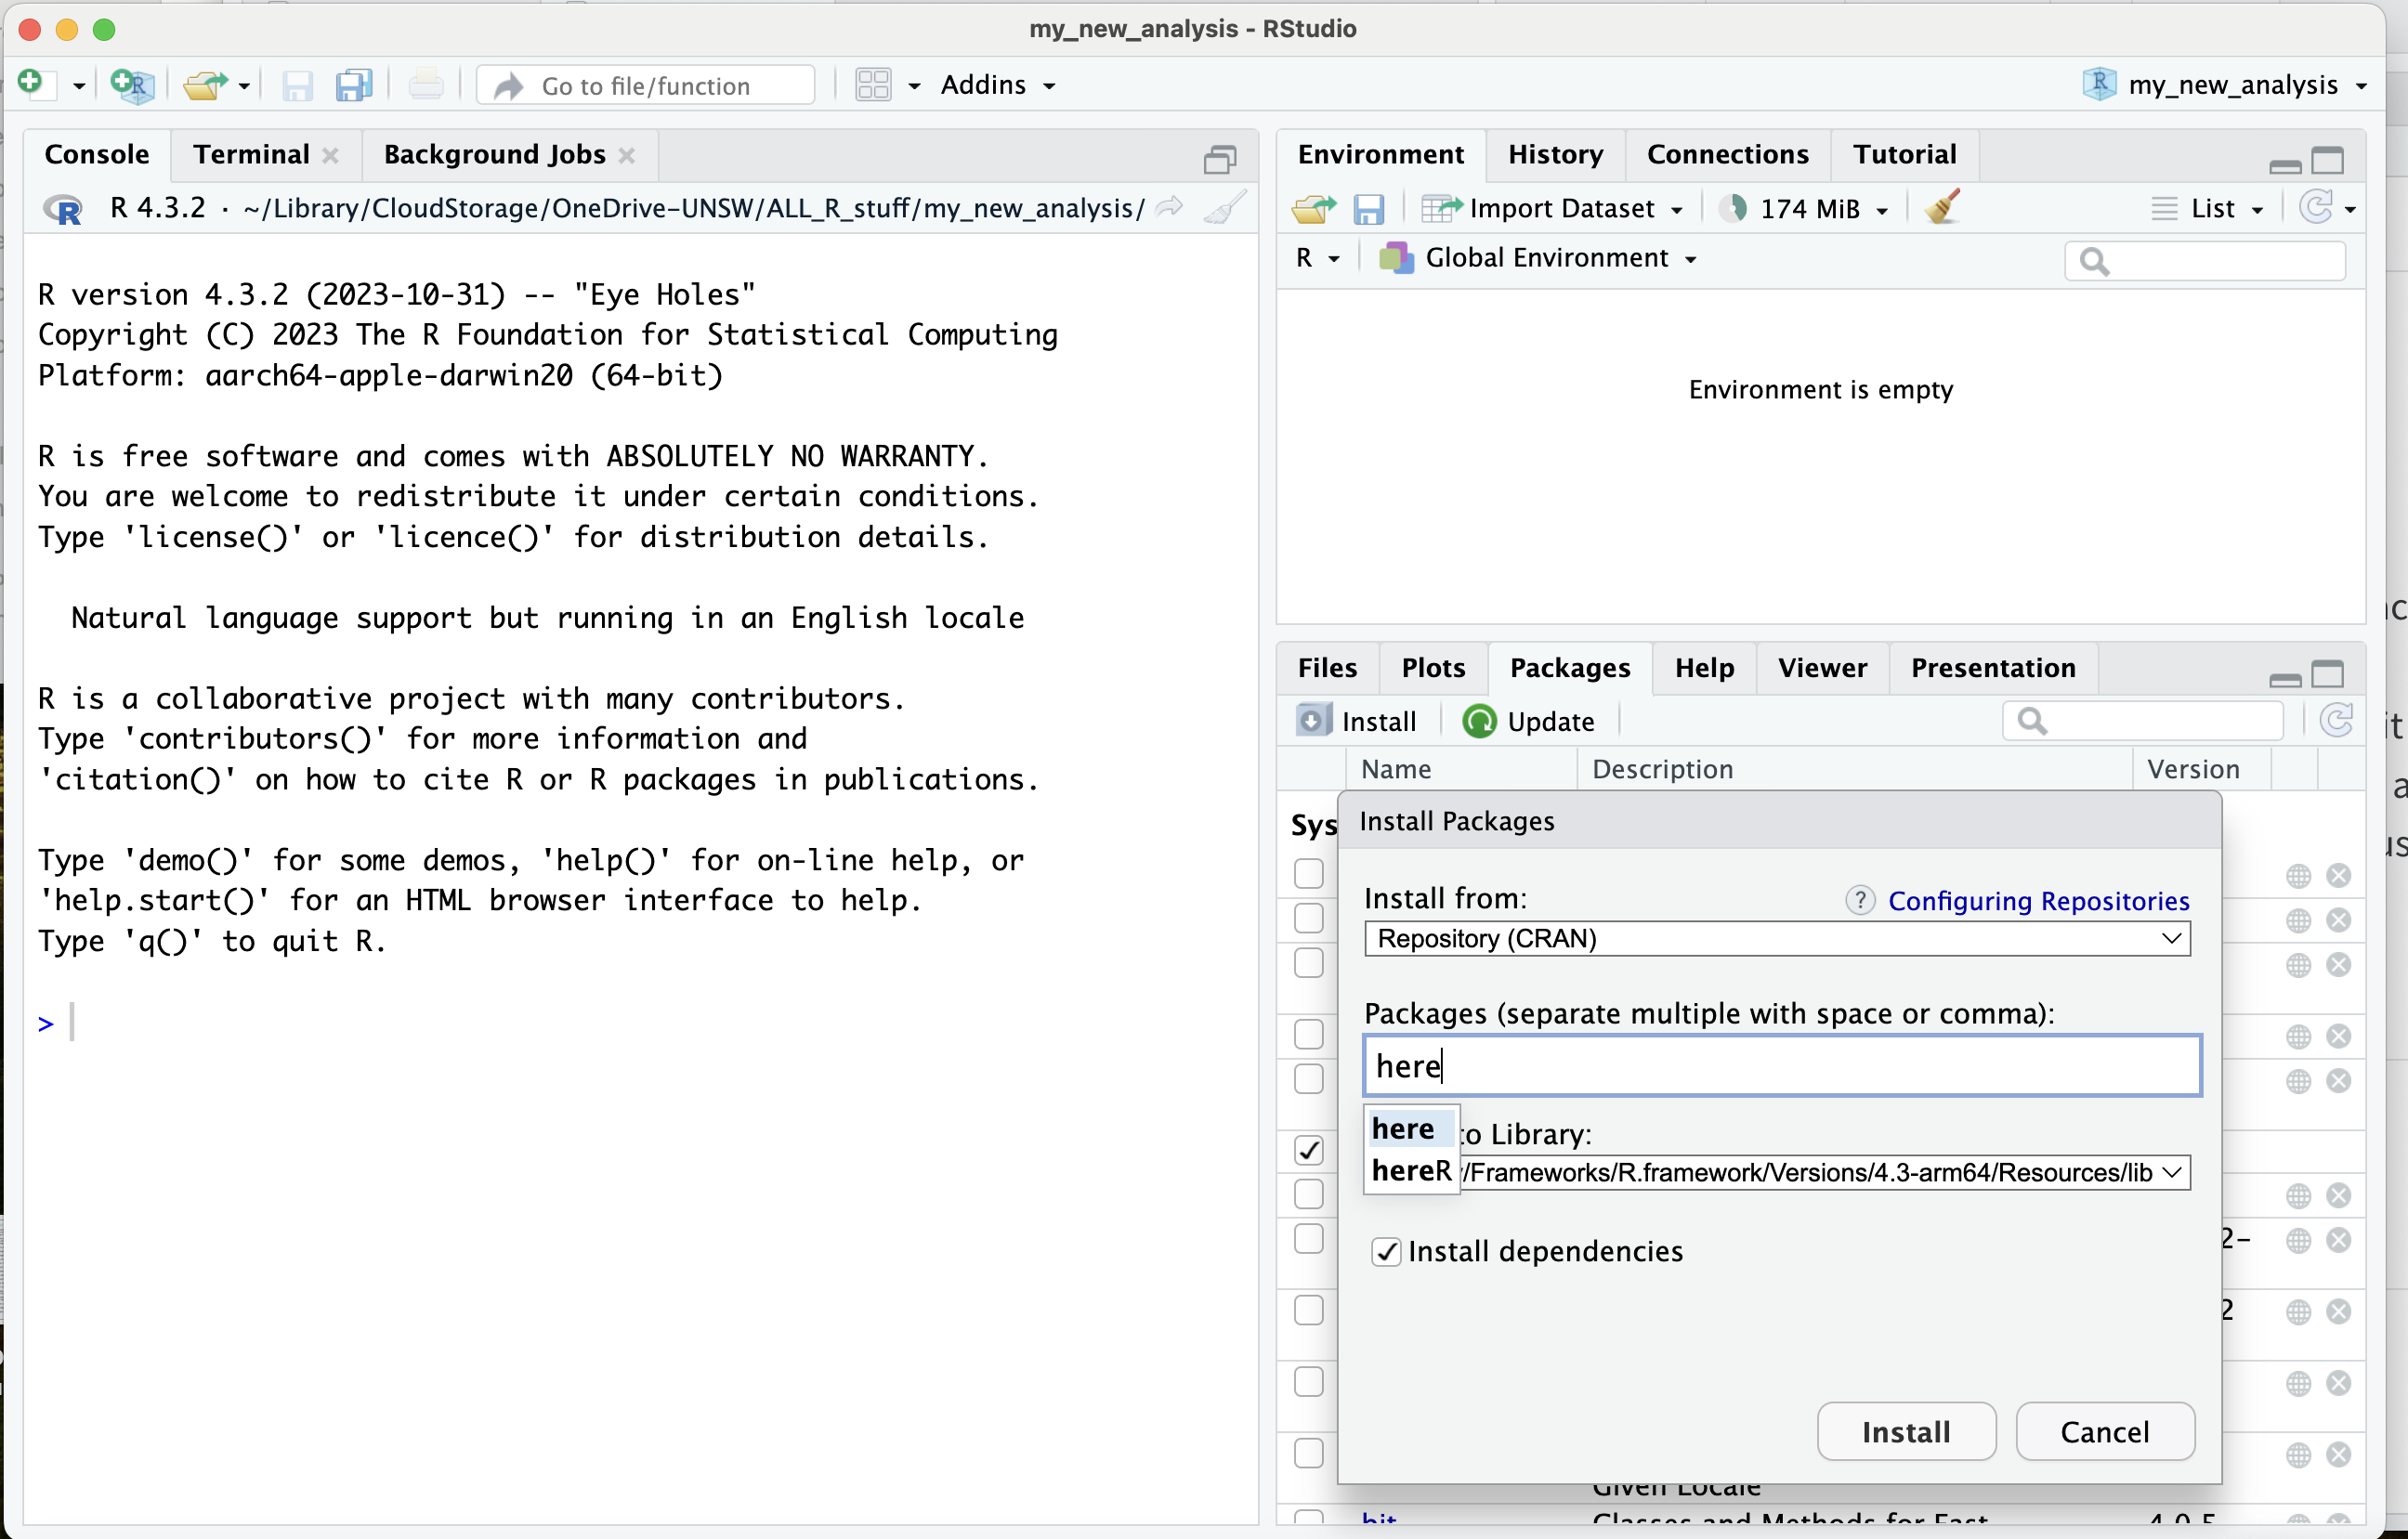
\includegraphics{images/install.png}

}

\caption{You can search for packages and install them from CRAN via the
packages tab}

\end{figure}%

\begin{quote}
Remember once you have installed a package, you will need to use the
\texttt{library()} function to load it before it will work.
\end{quote}

\section{useful packages for
psychology}\label{useful-packages-for-psychology}

\begin{itemize}
\tightlist
\item
  \texttt{tidyverse} this is a cluster of super helpful data wrangling
  and visualisation tools.
\item
  \texttt{here} this package helps direct R to the correct place for
  files based on the current working directory.
\item
  \texttt{janitor} this package helps us clean up data - especially
  awkward variable names.
\item
  \texttt{qualtRics} this package is helpful in reading in data files
  from Qualtrics\ldots{} except for .sav SPSS format files! (see next)
\item
  \texttt{haven} this package is a good one for reading in .sav SPSS
  format files
\item
  \texttt{sjplot} this package is helpful for making a `codebook' of
  your variables and values from imported .sav files
\item
  \texttt{surveytoolbox} this package is helpful in drawing out the
  value labels of variables imported in .sav format -- note: because
  \texttt{surveytoolbox} is on github and not CRAN, you'll want to do
  the following two steps \emph{in the console}. Note that we do this in
  the console since we only need to do it once! If the install asks you
  about updating packages, go ahead and do it! ---(1) install the
  \texttt{devtools} package: install.packages(``devtools'') ---(2)
  install via github:
  devtools::install\_github(``martinctc/surveytoolbox'')
\item
  \texttt{ufs} this package (short for user friendly science) is a nice
  tool for computing the internal reliability of scales -- note: one of
  the commands we will use in \texttt{ufs} requires the \texttt{psych}
  package to be installed (but doesn't need to be loaded via
  \texttt{library()}). Ensure you install that first. Two steps: ----(1)
  install the `remotes`` package: install.packages(``remotes'') ----(2)
  install via github\_lab: remotes::install\_gitlab(`r-packages/ufs')
\item
  \texttt{apa} nice for making statistical output into APA style
\item
  \texttt{gt} nice for making your tables look pretty
\item
  \texttt{apaTables} makes nice APA-styled tables of correlation, ANOVA,
  regression etc. output
\item
  \texttt{report} is a package to help with results reporting
\item
  \texttt{psych} is an umbrella package for lots of common psych tasks
\item
  \texttt{ez} is a great package for stats, including analysis of
  variance
\item
  \texttt{emmeans} is helpful for comparing specific means in a
  factorial design
\end{itemize}

\bookmarksetup{startatroot}

\chapter{using inline code}\label{using-inline-code}

\begin{quote}
JR maybe this piece needs to go in a separate chapter about writing with
RMarkdown, papaja etc
\end{quote}

\begin{Shaded}
\begin{Highlighting}[]
\CommentTok{\#pulls from the exclusions\_summary tabyl created above}

\NormalTok{comments\_only\_count }\OtherTok{\textless{}{-}}\NormalTok{ exclusions\_summary }\SpecialCharTok{\%\textgreater{}\%} \FunctionTok{filter}\NormalTok{(exclude\_coded }\SpecialCharTok{==} \StringTok{"comments only"}\NormalTok{) }\SpecialCharTok{\%\textgreater{}\%} \FunctionTok{pull}\NormalTok{(n)}
\NormalTok{comments\_only\_count2 }\OtherTok{\textless{}{-}}\NormalTok{ exclusions\_summary}\SpecialCharTok{$}\NormalTok{n[}\FunctionTok{which}\NormalTok{(exclusions\_summary}\SpecialCharTok{$}\NormalTok{exclude\_coded}\SpecialCharTok{==}\StringTok{"comments\_only"}\NormalTok{)]}

\NormalTok{time\_only\_count }\OtherTok{\textless{}{-}}\NormalTok{ exclusions\_summary }\SpecialCharTok{\%\textgreater{}\%} \FunctionTok{filter}\NormalTok{(exclude\_coded }\SpecialCharTok{==} \StringTok{"time only"}\NormalTok{) }\SpecialCharTok{\%\textgreater{}\%} \FunctionTok{pull}\NormalTok{(n)}
\NormalTok{variance\_only\_count }\OtherTok{\textless{}{-}}\NormalTok{ exclusions\_summary }\SpecialCharTok{\%\textgreater{}\%} \FunctionTok{filter}\NormalTok{(exclude\_coded }\SpecialCharTok{==} \StringTok{"variance only"}\NormalTok{) }\SpecialCharTok{\%\textgreater{}\%} \FunctionTok{pull}\NormalTok{(n)}
\NormalTok{total }\OtherTok{\textless{}{-}}\NormalTok{ exclusions\_summary }\SpecialCharTok{\%\textgreater{}\%} \FunctionTok{filter}\NormalTok{(exclude\_coded }\SpecialCharTok{==} \StringTok{"Total"}\NormalTok{) }\SpecialCharTok{\%\textgreater{}\%} \FunctionTok{pull}\NormalTok{(n)}
\NormalTok{kept }\OtherTok{\textless{}{-}}\NormalTok{ exclusions\_summary }\SpecialCharTok{\%\textgreater{}\%} \FunctionTok{filter}\NormalTok{(exclude\_coded }\SpecialCharTok{==} \StringTok{"kept"}\NormalTok{) }\SpecialCharTok{\%\textgreater{}\%} \FunctionTok{pull}\NormalTok{(n)}
\end{Highlighting}
\end{Shaded}

Use of inline code is really helpful in avoiding transcription errors
and saving time when writing up! Here, we use code to pull in some
descriptive statistics from the exclusion reason table we made above:

\begin{quote}
INSERT INLINE EXAMPLE HERE
\end{quote}

\bookmarksetup{startatroot}

\chapter{helpful console commands}\label{helpful-console-commands}

\begin{itemize}
\tightlist
\item
  names(objectname) - returns a list of variable names for that
  dataframe, making it less likely you will type things incorrectly
\item
  getwd() - returns the path to the current working directory. Run this
  in the console.
\item
  rm(objectname) - removes the object from your global environment. Can
  be helpful in cleaning up any `test' objects you make while
  troubleshooting code.
\item
  ?package - brings up the Help info for that package
\item
  ?function - brings up the Help info for that function
\end{itemize}

\bookmarksetup{startatroot}

\chapter{useful keyboard shortcuts}\label{useful-keyboard-shortcuts}

Option-Command-I = inserts a new code chunk Command-Enter = runs the
chunk of code that your cursor is in

\bookmarksetup{startatroot}

\chapter{commonly encountered errors}\label{commonly-encountered-errors}

\bookmarksetup{startatroot}

\chapter*{References}\label{references}
\addcontentsline{toc}{chapter}{References}

\markboth{References}{References}

\phantomsection\label{refs}
\begin{CSLReferences}{0}{1}
\end{CSLReferences}



\end{document}
